\chapter{Detaljeløsning} \label{Detaljeløsning}
Detaljeløsningen er opdelt i afsnit, der hver har til formål, at udvikle løsningen på baggrund af præstationskravene, der beskrives i starten af hvert afsnit. Kapitlet starter med en præsentation af løsningen. Igennem detaljeløsningen foretages valg af materiale, dimensionering og design, baseret på kinematiske og statiske beregninger, samt undersøgelse af standardkomponenter. Kapitlet afsluttes med gennemgang af produktion, prissætning og opsummering af præstationskrav. Relevante valg og resultater opsummeres i slutningen af hvert afsnit, enten med tabeller, figurer eller tekst.   

%Det endelige koncept fra \ref{Endelig koncept} videreudvikles i dette kapitel til en løsning der beskrives i afsnit \ref{Produkt}. Kapitlet gennemgår design og materialevalg med udgangspunkt i præstationskravene fra afsnit \ref{tab:basale krav}. I sektion \ref{Materialevalg} redegøres for valg af materiale. 
%I sektion \ref{farvedispensering med PeJV} vil det blandt andet fastlægges hvilken PeJV som benyttes, på baggrund af relevante designspecifikationer, herunder prikstørrelse, variation af prikstørrelse, antal påføringsmidler, kontrast og opstart på tidsforbrug. I sektion \ref{Præcision af prikplacering} vil produktet undersøges for præcision ved beregninger, herunder afvigelse af prikplacering, samt tidsforbrug pr. cm\(^2\) ved en kinematisk analyse. I sektion \ref{Valg af led screw og motor} udvælges standard komponenter. Stellet dimensioneres efter disse. De bevægelige dele bliver også her designet med fokus på, at kunne nå alle steder indenfor arbejdsområdet, samt at danne overblik over mængden af almindelig- og specialværktøj, som benyttes. I \ref{Indspænding} designes indspændingen med fokus på at reducere bevægeligheden af det indspændte emne, samtidig med, det er et simpelt design, som skal mindske tiden brugt på opsætning. I \ref{Produkt} præsenteres CAD-tegningerne af hele produktet, samt fremstillingsmetoder og en stykliste og prisestimat. I \ref{vurdering af krav} vurderes alle præsentationskravene fra \ref{tab:basale krav} imod det endelige produkt, samt vurdering af brugerinvolvering under prikprocessen


%\plainbreak{2}
%\section{Materialevalg} \label{Materialevalg}

Ved udviklingen af en robot til præcis påføring af speckle pattern, bliver det nødvendigt at vurdere forskellige materialer ud fra både mekaniske og praktiske egenskaber. Formålet med dette afsnit er at undersøge, hvilke materialer, der bedst kan opfylde kravene til stivhed, styrke, lav vægt, slidstyrke, og bearbejdelighed. Tre materialer, der fremstår som særligt relevante i denne sammenhæng er aluminium (EN AW-6082 T6), rustfri AISI 304 stål og kulfiberforstærket polymer (CFRP). Disse materialer repræsenterer hver deres styrker og svagheder, og det er derfor væsentligt at analysere deres egenskaber i forhold til konstruktionens funktionelle krav.

%Aluminium EN AW-6082 T6 er et let metal med en densitet på cirka 2700 kg/m\(^3\) og et E-modul omkring 71 GPa. Aluminiumet tilbyder et gunstigt forhold mellem vægt og stivhed, hvilket gør det velegnet til strukturer, hvor lav masse og tilstrækkelig mekanisk styrke er væsentlige krav. Materialets flydespænding er 255 MPa, og dets trækstyrke spænder  fra 300 til 340 MPa.  EN AW-6082 T6 har desuden gode bearbejdningsegenskaber, idet det let kan fræses, bores og svejses. En yderligere fordel er dets naturlige korrosionsbestandighed, hvilket reducerer behovet for omfattende overfladebehandling i mange anvendelser. Aluminium er samtidig relativt økonomisk tilgængeligt med en gennemsnitlig pris på omkring 244 DKK pr. kilogram \parencite{Aluminiumplade}. Ulempen ved aluminium er dog, at materialet i visse tilfælde kan have begrænset modstandskraft over for høje punktbelastninger, hvilket kan føre til lokal plastisk deformation, hvis konstruktionen ikke dimensioneres tilstrækkeligt.\parencite{Hesse2011AluminiumSheets}.

Rustfri AISI 304 stål er et materiale med væsentligt højere densitet, omkring 7900 kg/m\(^3\), og en E-modul på cirka 193 GPa. Stål tilbyder en betydeligt højere stivhed og styrke end aluminium, hvilket gør det særligt egnet til komponenter, som udsættes for store belastninger eller gentagen mekanisk påvirkning. flydespænding for almindelige konstruktionsstål ligger typisk omkring 215 MPa, mens trækstyrken ligger mellem 500 og 750 MPa. Denne høje styrke gør stål velegnet til områder, hvor strukturel integritet og dimensionsstabilitet er afgørende over lang tid. Dog medfører den høje masse, at stålkonstruktioner i bevægelige systemer kan føre til øgede krav til motorstørrelser og energiforbrug. Stål tillader nøjagtig maskinbearbejdning og tilbyder robuste svejseegenskaber, hvilket kan være en fordel i konstruktioner, hvor stor præcision og høj samlingsstyrke er påkrævet. Prisen på stål ligger relativt lavt i forhold til andre materialer, med en gennemsnitlig pris på omkring 79 DKK pr. kilogram \parencite{Stalprofil}, hvilket gør det attraktivt i applikationer, hvor vægt ikke er den primære begrænsning \parencite{Jessen2011RustfritKorrosion}.

Kulfiberforstærket polymer (CFRP) skiller sig væsentligt ud fra metallerne ved at kombinere en meget lav densitet, typisk omkring 1600 kg/m\(^3\), med en meget høj mekanisk styrke i fiberretningen. E-modulet for CFRP varierer typisk mellem 70 og 140 GPa afhængigt af fiberindhold og opsætning, mens trækstyrken i fiberretningen ofte ligger mellem 600 og 1200 MPa. Dette giver mulighed for ekstremt lette og stive strukturer, som kan bevæge sig hurtigt og præcist med minimale inertikræfter. CFRP er dog anisotropt, hvilket betyder, at dets mekaniske egenskaber afhænger stærkt af fiberorienteringen, og materialet kan være følsomt over for belastninger på tværs af fibrene. Derudover er bearbejdning af kulfiber mere kompliceret end for metaller, og processen kræver specialværktøj og særlige sikkerhedsforanstaltninger for at håndtere støv og fibre korrekt. Økonomisk ligger CFRP væsentligt højere end både aluminium og stål, med en gennemsnitlig pris på omkring 800–1200 DKK pr. kilogram, hvilket begrænser dets anvendelse til applikationer, hvor materialets unikke kombination af lav vægt og høj stivhed er afgørende\parencite{Starr1995CarbonDatabook}.


\begin{comment}
    \begin{table}[H]
    \centering
    \caption{Materialeegenskaber}
    \begin{tabular}{|l|c|c|c|} \cline{2-4}
        \multicolumn{1}{c|}{~} & \rowcolor{lightgray!20} Aluminium & Stål & CFRP \\ \hline
        \multicolumn{1}{|l|}{ \cellcolor{aaublue} \textcolor{white}{E-modul}} & 69 GPa & 210 GPa & 70-140 GPa\\ \hline
        \multicolumn{1}{|l|}{\cellcolor{    aaublue} \textcolor{white}{Flydespænding $\sigma_y$}}& 190-210 MPa& 355 MPa&  -\\ \hline
        \multicolumn{1}{|l|}{\cellcolor{aaublue} \textcolor{white}{Trækstyrke}} & 215-250 MPa& 470-630 Mpa& 1000 MPa \\ \hline
        \multicolumn{1}{|l|}{\cellcolor{aaublue} \textcolor{white}{Densitet $\rho$}}& 2700 $kg/m^{3}$ & 7850 $kg/m^{3}$ & 1600 $kg/m^{3}$\\ \hline
    \end{tabular}
\end{table}
\end{comment}



\begin{table}[H]
    \centering
    \footnotesize
    \caption{Materialeegenskaber}
    \begin{tabular}{|l|c|c|c|c|c|} \cline{2-5}
        \multicolumn{1}{c|}{~} & \multicolumn{1}{|c|}{ \cellcolor{aaublue} \textcolor{white}{E-modul}} &  \multicolumn{1}{|c|}{\cellcolor{aaublue} \textcolor{white}{\textbf{Flydespænding $\sigma_y$}}} & \multicolumn{1}{|c|}{\cellcolor{aaublue} \textcolor{white}{Trækstyrke $\sigma_{TS}$}} & \multicolumn{1}{|c|}{\cellcolor{aaublue} \textcolor{white}{Densitet $\rho$}} & \multicolumn{1}{|c|}{\cellcolor{aaublue} \textcolor{white}{Pris pr. kg}}\\ \hline
        
         \multicolumn{1}{|l|}{\cellcolor{lightgray!20}{EN AW-6082 T6}} & 71 GPa & 255 MPa & 300-340 MPa & 2700 $\frac{kg}{m^3}$ & 244 DKK\\ \hline
         
        \multicolumn{1}{|l|}{\cellcolor{lightgray!20}{Rustfri AISI 304 stål}} & 193 GPa & 215 MPa & 500-750 MPa & 7900 $\frac{kg}{m^3}$ & 79 DKK \\ \hline
        
        \multicolumn{1}{|l|}{\cellcolor{lightgray!20}{CFRP}} & 70-140 GPa & - & 1000 MPa &  1600 $\frac{kg}{m^3}$ & 800-1200 DKK \\ \hline
    \end{tabular}
    \label{tab:materialeegenskaber}
\end{table}

Sammenfattende viser vurderingen, at materialernes anvendelighed afhænger nøje af de specifikke krav til den enkelte komponent i robotten. EN AW-6082 T6  tilbyder en fordelagtig kombination af lav vægt, god bearbejdelighed og moderat styrke. konstruktionstål giver høj stivhed og styrke til en lav pris, men med en øget vægt. Kulfiberforstærket polymer fremstår som det letteste og mest stive alternativ i bestemte retninger, men til en høj materialepris og med begrænsninger i forhold til bearbejdning og genanvendelse. Grundet dets høje pris og omfattende fremstilling fravælges CFRP. Derfor vælges det at robotten skal fremstilles i EN AW-6082 T6 og stål. Her vælges det at størstedelen af konstruktionen skal produceres i aluminium, og sliddele skal produceres i stål for at øge produktets levetid.


%- Erstatte alu med plast i dele vi selv har designet \\

\plainbreak{2}
\section{Løsning til speckle pattern robot} \label{Produkt}
Produktet fungerer ved, at emnet placeres på arbejdspladen, hvorefter emnet manuelt indspændes. Bevægelsen på x-aksen drives af en motor, som roterer en ledeskrue, hvorpå der bevæges en vogn frem og tilbage og understøttet af følgestænger. Motorerne som driver x-aksen og ledeskruerne, er monteret til en indspændingsblok, som sørger for at følgestængerne fastholdes. Indspændingsblokken er fast monteret til et stel. Stellet består af en kombination af aluminium ekstruderet t-slots i forskellige længder. I ledeskruernes modsatte ende sidder yderligere en indspændingsblok, som både fastspænder følgestængerne og indeholder et kugleleje til ledeskruen. For at opnå bevægelse på y-aksen, er der monteret en motor på x-aksens ene vogn og en kontra vægt på den anden vogn. Mellem de to vogne udspændes yderligere en ledeskrue og to følgestænger, som driver en vogn, der har PeJV'en monteret. Vognen på y-aksen er udformet så PeJV'en kan justeres manuelt i højden, for at passe til forskellige emne højder. 
\begin{figure}[H]
    \centering
    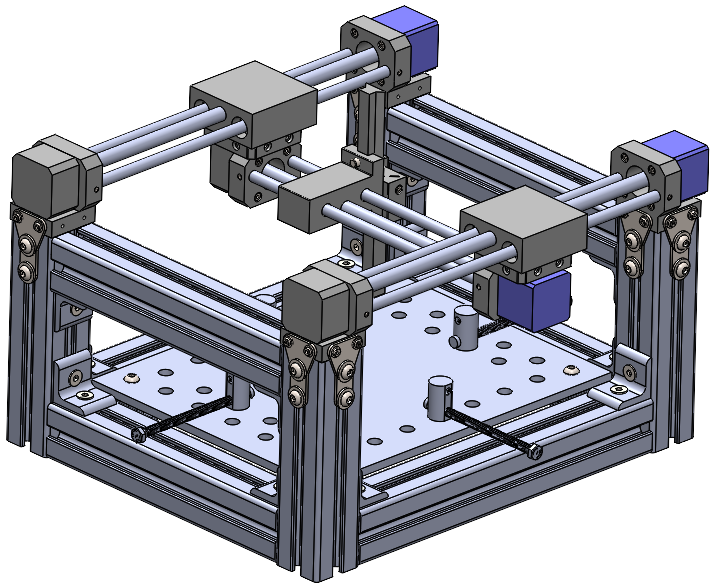
\includegraphics[width=0.7\linewidth]{Sections/6 Detaljeløsning/Media/final assembly.png}
    \caption{Illustration af løsning, med markering af vigtigste dele}
    \label{fig: skitse med navne}
\end{figure} \plainbreak{-1}

 



\plainbreak{2} 
\section{Farve dispensering med PeJV} \label{farvedispensering med PeJV}

Det er i afsnit \ref{Prikplacering} valgt, at anvende en PeJV til farvedispensering. Projektet er afgrænset fra undersøgelse af specifikke farvetyper, men for at opfylde præstationskravene vælges en bestemt PeJV, som løsningen udvikles til. Følgende præstationskrav fra tabel \ref{tab:basale krav}, danner grundlag for vurderingen af en PeJV:
%Udvælgelsen af en specifik PeJV afhænger af præstationskravene givet i tabel  hvor krav nr. 1, 2, 6, 7, samt 8. Ud fra disse parametre skal en PeJV udvælges: Kravene lyder således:
\begin{itemize}
    \item[1.] Justerbar prikstørrelse fra \(\SI{0,1}{mm}\) - \(\SI{1,0}{mm}\)
    \item[2.] Variation i størrelse af påsat prik på maksimalt $\SI{\pm0,05}{mm}$ 
    \item[6.] Mængde af forskellige farvemidler til koncept på minimum 2
    \item[8.] Maksimalt tidsforbrug på prikplacering pr. cm\(^2\) på 30 sekunder
\end{itemize}

Til projektet er det valgt, at anvende DV-6200-serien fra VIEWEG, hvor der tages udgangspunkt i DV-6210, som kan ses på figur \ref{fig:Jetventil}, for at have specifikke tal at regne på. Denne serie er udvalgt da de er opgivet til at kunne dispensere mængder i sub-nanoliter. Hvis den placerede dråbe forbliver en halvkugle på overfladen, er det muligt at undersøge den volumen prikværktøjet skal udskyde, for at opnå en radius på $\SI{0,1}{mm}$ eller under. \parencite{VIEWEG2025JetDV-6210}

\begin{equation}
    V=\dfrac{4}{3}\cdot \pi\cdot r^3
\end{equation}

Her udregnes det, at en volumen under \SI{4,2}{nL}, giver en radius på \SI{0,1}{mm}, og det vides at der kan dispenseres mindre end dette. Det er altid muligt at lave større prikker, da værktøjet kan dispensere flere prikker på samme sted. Prikværktøjet godkender præstationskrav 1 om prikstørrelse.
Baseret på produktets tekniske dokumentation vurderes det er opfylde præstationskrav 2. Det vurderes, at DV-6210'eren kan dispensere forskellige farvemidler, da den er designet til at dispensere syre, baser og olier. Tidsforbruget pr. cm\(^2\) afhænger af bevægelseshastigheden og dispenseringsfrekvensen. DV-6210 kan dispensere med op til \SI{3000}{Hz} og det vurderes dermed, at dette ikke blive den begrænsende faktor i hastigheden af produktet.

\begin{figure}[H]
    \centering
    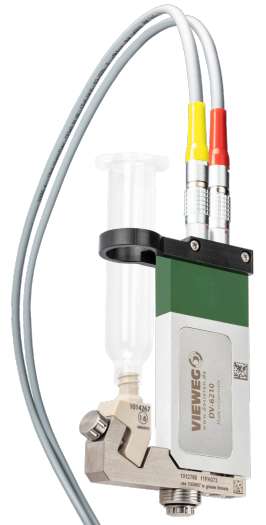
\includegraphics[width=0.25\linewidth]{Sections/6 Detaljeløsning/Media/Jetventil DV1.png}
    \caption{Billede af Jet valve DV-6210 fra: \parencite{VIEWEG2025JetDV-6210}.}
    \label{fig:Jetventil}
\end{figure}
\plainbreak{-0.5}

%Størrelsen af farvedråben på emnet, afhænger af farvemidlet, der benyttes til emnet, men dysehovedets åbning er udskiflig og kan købes med en diameter fra 0.03 mm til 1.2 mm. Det er derved blevet vurderet at Jet valve DV-6210 er et passende valg til produktet. 

Et komplet sæt Jet Valve DV-6210 fra VIEWEG inklusiv pumpe, kontrolsystem og dysehoveder koster €8.385 ($\approx 62.500 DKK$). Dens minimale vægt er \SI{260}{g}, uden farvemiddel. \parencite{VIEWEG2025JetDV-6210}. 


\renewcommand{\arraystretch}{1.3}
\begin{table}[H]
\setlength{\tabcolsep}{20pt}
 \centering
  \caption{Opsummering}
 \begin{tabular}{|c c|} \hline
 \multicolumn{2}{|c|}{\cellcolor{aaublue} \color{white} \textbf{VIEWEG DV-6210}}  \\\hline
 \rowcolor{gray!10} \multicolumn{1}{|c}{\textbf{Variabel}} &  \multicolumn{1}{c|}{\textbf{Værdi}}  \\\hline
 
 %PeJV &  VIEWEG DV-6210\\\hline
 Vægt &  $\geq \SI{260}{g} $\\\hline
 Minimal diameter på prikstørrelse &  $\diameter\SI{0,08}{mm}$\\\hline
 Prikker pr. sekund &  3000 \\\hline
 \end{tabular}
 \label{tab: PeJV opsummering}
\end{table}

%(skulle have stået mellem linje 19 go 21)%PeP blev fravalgt på baggrund af manlgede forsknings artikler og indrustri brug, af PeP dråbe dosering. Derudover blev PeJV valgt frem for TIJ, grundet den højere hastighed, der kan opereres med.

\plainbreak{2}
\section{Nøjagtighed af prikplacering} \label{Præcision af prikplacering}

Nøjagtigheden af løsningen er betydelig, for at produktet kan opfylde følgende præstationskrav:

\begin{itemize}
    \item[3.] Variation på prikplacering på \(\SI{\pm0.1}{mm}\)
    \item[8.] Tidsforbrug på prikplacering pr. cm$^2$ på 30 sekunder
\end{itemize}

De lineære aksers bevægelse undersøges i en kinematisk analyse i afsnit \ref{Kinematisk analyse}, hvor variation på prikplacering og tidsforbruget estimeres. 

%Der undersøges hvordan de lineære bevægelser opfører sig i den kinematiske analyse i afsnit \ref{Kinematisk analyse}. Tidsmæssigt må det ikke tage mere end 30 sekunder for produktet at producere én cm\(^2\). 

%Dette kommer fra præstationskravene i tabel \ref{tab:basale krav}. 


\subsection{Valg af ledeskrue} \label{Valg af led screw og motor}
Det er i afsnit \ref{løsningsanal: Lineær bevægelse} valgt, at benytte en ledeskrue til de lineære bevægelser. Det er nødvendigt, at finde dimensioner på ledeskruen, samt dens gevindhældning, for at beregne variation på prikplacering og tidsforbruget, da disse afhænger af hældningen på gevindet. 
Gevindhældningen er den lineære afstand gevindet har bevæget sig ved en omgang, og er illustreret i figur \ref{fig: skrue forklaringer}. En højere gevindhældning vil resultere i længere lineær bevægelse per omgang. Det medfører også en lavere præcision, da en motor er begrænset i, hvor lille en vinkel den kan rotere sig.


\begin{figure}[H]
    \centering
    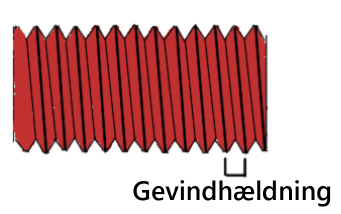
\includegraphics[width=0.4\linewidth]{Sections/6 Detaljeløsning/Media/skruer.png}
    \caption{Illustration gevindhældning}
    \label{fig: skrue forklaringer}
\end{figure} \plainbreak{-0.5}

Nøjagtigheden er også afhængig af motoren, både i forhold til eventuelle unøjagtigheder i motorens konstruktion, samt den mindste rotation den kan udføre. Da løsningen kommer til at skulle foretage mange små og præcise bevægelser kan der allerede nu konkluderes at en step-motor er bedst egnet til formålet. step-motorer rotere i steps i stedet for kontinuert, som en servomotor, dette betyder det er muligt at nøjagtigt kontrollere hvor meget motoren skal rotere. En fuld rotation er delt op i et antal steps, dette kaldes \textit{step antal}. Nogen fabrikanter vælger i stedet at oplyse hvor mange grader et step dækker, dette kaldes \textit{stepvinkel}

Grundet de geometriske begrænsning vælges det at motoren skal være af typen NEMA 14. Dette er en monterings standard fra National Electrical Manufacturers Association (NEMA). Denne størrelse motor har typisk en step antal på 200, og det er dette ledeskrue dimensioneres ud fra.

I HoQ blev der konkluderet at nøjagtighed er vigtigere end hastighed.  For at tage hensyn til begge kravs vigtighed, vælges der en ledeskrue med en gevindhældning på \SI{2}{mm}. Dette giver en maksimal afvigelse på \SI{0,01}{mm}, som opfylder præstationskrav 3 med en sikkerhedsfaktor på 10. Det vælges derudover, at skruen skal have en diameter på \SI{10}{mm}, da det vil give en større modstand imod udbøjning. \parencite{Igus2025DrylinSteel}




%Når gevindstigningen nævnes, menes der afstanden imellem hvert indhak i gevindet. Dette er det samme som gevindhældningen i tilfældet af, at skruen er en enkeltstartsskrue. Dette betyder at der skrues langs én linje i skruen, hvorimod dobbeltstart har to parallelle linjer på skruen der skrues langs, som det ses på figur \ref{fig: skrue forklaringer}. \parencite{Sild2022LeadFractory} 

\plainbreak{2}

\subsection{Kinematisk analyse af lineær bevægelse} \label{Kinematisk analyse}
Løsningen skal sætte prikker i et arbejdsområde på \SI{200}{mm} \(\times\) \SI{150}{mm} \(\times\) \SI{50}{mm} område, hvor det ønskes, at robotten kan opnå en vilkårlig position indenfor dette område. I dette afsnit undersøges, hvordan PeJV'en skal bevæge sig, for at opfylde dette. Heraf skal PeJV'en bevæges i x-og y-retningen. Der kræves en høj præcision, i og med at en påsat prik kun må afvige med $\SI{\pm0,1}{mm}$ for at opfylde præstationskrav 1.
%Robotten skal bevæge sig i både x-og y-retningen, for at udføre sin opgave. Løsningen er den samme for de bevægelige dele i både x-og y-retningen. Drivmidlet for bevægelsen er en Nema 14 stepper motor, som sammen med en ledeskrue skaber bevægelsen. Motoren udføre et drejningsmoment på maks \(0,2\)Nm og roterer op til 2000 RPM, som sætter gang i rotationen af ledeskruen. Motoren er en stepper motor, hvilket betyder at den rotere i små steps. Én rotation er lig 360\(\degree\) og motoren har en step vinkel på 1,8\(\degree\), altså har motoren 200 steps for at opnå én rotation. Ledeskruen har en gevindstigning på \(2\)mm og en gevindhældning på \(2\)mm. 

Løsningen er den samme for de bevægelige dele i både x-og y-retningen i et kartesisk koordinatsystem. De lineære bevægelser der designes til løsningen, benævnes \textit{ Lineær x-akse} og \textit{Lineær y- og z-akse}, for bevægelsen der henholdsvis sker parallel med x-aksen og y-aksen. Disse fremgår af figur \ref{Skite af akser med pile}, hvor bevægelsesretningen er angivet med blå pile, og ledeskruernes rotation med røde pile

\begin{figure}[H]
    \centering
    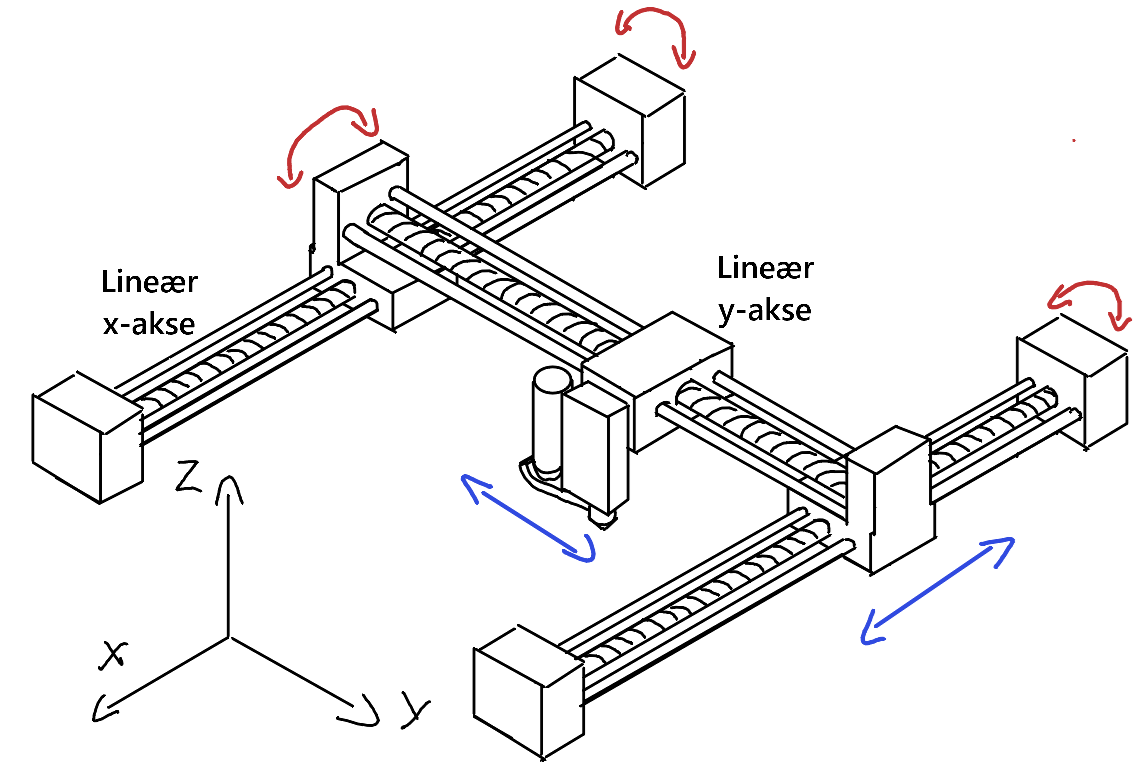
\includegraphics[width=0.8\linewidth]{Sections/6 Detaljeløsning/Media/Akser med pile.png}
    \caption{Skitse af akser, med bevægelsesretninger for de lineære akser angivet med blå pile, og ledeskruernes rotation med røde pile.}
    \label{Skite af akser med pile}
\end{figure}

Drivmidlet for bevægelsen i x-og y-aksen er en step-motor, som sammen med den udvalgte ledeskrue skaber bevægelsen. Motoren skaber et drejningsmoment, som sætter gang i rotationen af ledeskruen, der skubber to vogne langs x-aksen og PeJV'en langs y-aksen. Hvor meget akserne bevæger sig, er bestemt ud fra gevindhældningen af ledeskruen. Ledeskruen er udvalgt og i dette afsnit undersøges hvilken motor, som skal benyttes.


\begin{figure}[H]
    \centering
    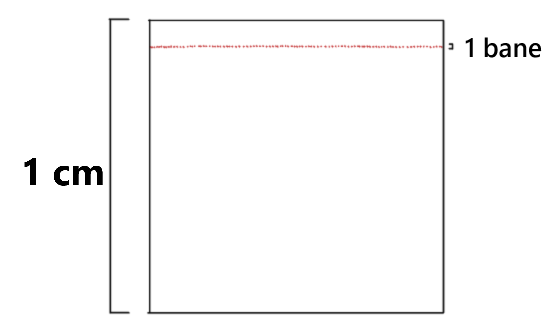
\includegraphics[width=0.4\linewidth]{Sections/6 Detaljeløsning/Media/Bane.png}
    \caption{Skite af én bane}
    \label{fig: Skite bane}
\end{figure}

I bilag \ref{Bilag - Bevægelse} gennemgås udledningen af en formel for tid pr. cm\(^2\), men også en formel for tiden det tager at køre én bane (se figur \ref{fig: Skite bane}).
En bane er defineret ud fra kvadratcentimeterens dimensioner. Da prikværktøjet kan sætte prikker under bevægelse, vil den kunne sætte en række af prikker på den tid den kan bevæge sig igennem rækken. Tiden det tager prikværktøjet at lave en række prikker fra den ene side af kvadratcentimeteren til den anden, kaldes banetiden. Banen kan ses på figur \ref{fig: Skite bane}. Prikkerne har som minimum en diameter på $\SI{0,1}{mm}$, og det er derfor muligt at placere højest 100 prikker på langs af \SI{1}{cm}, for at placere prikker på hele kvadratcentimeteren. Det er altså nødvendigt at lave 100 baner med $\SI{0,1}{mm}$ prikker af \SI{10}{mm}, for at fylde hele kvadratcentimeteren med prikker. Dette er anslået til den maksimale tid det vil tage at prikke en kvadratcentimeter, og vil bruges som overslag til tiden det vil tage at lave et speckle pattern per kvadratcentimeter.

Motoren skal igennem tre faser for at udføre sin bevægelse på én bane, henholdsvis acceleration, konstant hastighed (top hastighed) og deceleration. Dette kan skrives som:
\begin{equation}
    t_{bane}=2\cdot t_{acc}+t_{top}
\end{equation}

Hvor \(t_{bane}\) er den samlede tid det tager produktet at bevæge sig én bane. \(t_{acc}\) er tiden det tager at accelerere, men også tiden det tager og decelerere, da denne værdi er den samme, ganges denne værdi med 2. Dette udtryk udledes i \ref{Bilag - Bevægelse} til:
\begin{equation}
    t_{bane}=\dfrac{m_{l}\cdot r_{l}^2\cdot \omega}{\tau}+\dfrac{s_{bane}}{\omega\cdot O}
    \label{eq: t_bane}
\end{equation}

I ligning \ref{eq: t_bane} er \(m_{l}\) massen af ledeskruen på \SI{136}{g}, \(r_{l}\) er radius af ledeskruen på \SI{5}{mm}, \(O\) er gevindhældningen af ledeskruen på \SI{2}{mm}. Motoren har to variabler i ligningen, henholdsvis \(\tau\) og \(\omega\), hvor \(\tau\) er drejningsmomentet produceret af motoren og \(\omega\) er vinkelhastigheden. Variablen \(s_{bane}\) er længden af én bane, hvor én bane i dette tilfælde er \SI{10}{mm}, da én cm\(^2\) er \SI{10}{mm} \(\times\) \SI{10}{mm}. Dette er grundet præstationskrav nr. 8 i tabel \ref{tab:basale krav} om tid pr. cm\(^2\) og derfor skal \(t_{bane}\) som nævnt tidligere ganges med 100 for at opnå én cm\(^2\). Denne værdi  kaldes \(t_{cm^2}\)
 \begin{equation}
      t_{cm^2}=\left(\dfrac{m_{l}\cdot r_{l}^2\cdot \omega}{\tau}+\dfrac{s_{bane}}{\omega\cdot O}\right) \cdot 100
      \label{eq:tcm2}
 \end{equation}

Det vurderes at motorens vinkelhastighed skal være så høj som muligt, da en højere top hastighed har større indflydelse på tiden end acceleration. \(\omega\) er den værdi, som er interessant grundet hastigheden af den roterende ledeskrue bestemmer hvor hurtigt x-og y-aksen bevæger sig. I og med kravet på tid pr. cm\(^2\) har en værdi på maksimalt 30 sekunder, og ikke er en ukendt variabel kan \(\tau\) isoleres. 
En funktion kan derved opsættes med \(\omega\) som variabel, så der kan aflæses en minimum vinkelhastighed, som skal benyttes for at produktet kan udføre sig arbejde:
\begin{equation}
    \tau(\omega)=\dfrac{m_{l} \cdot r_{l}^2 \cdot \omega}{t_{bane} \cdot O - s_{bane}}
\end{equation}

Denne funktion plottes i et koordinatsystem med \(\omega\) ud af x-aksen og \(\tau\) op af y-asken. En minimum værdi for \(\omega\) kan nu aflæses, se figur \ref{fig: Tau-Omega plot}:
\begin{figure}[H]
    \centering
    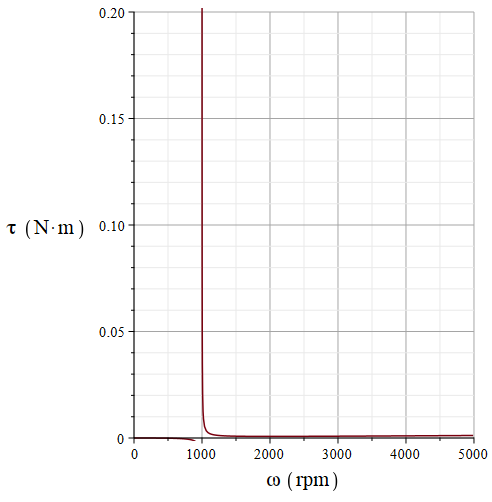
\includegraphics[width=0.5\linewidth]{Sections/6 Detaljeløsning/Media/Billeder til indspænding/tau-omegaplot.png}
    \caption{Graf over \(\tau\) som funktion af \(\omega\)}
    \label{fig: Tau-Omega plot}
\end{figure}

På figur \ref{fig: Tau-Omega plot} kan det ses at produktet vil kunne udføre sit arbejde, så længe \(\omega\) er over 1000 RPM. Kravet til valg af motor er således at den skal have en vinkelhastighed på minimum \SI{1000}{RPM} og med så højt drejningsmoment som muligt. Ud fra dette vælges en NEMA 14 step-motor. Den udvalgte motor sælges af firmaet Igus og har dimensionerne \SI{35}{mm} \(\times\) \SI{35}{mm} \(\times\) \SI{42}{mm} og kan levere et drejningsmoment op til \SI{0.18}{Nm} og en vinkelhastighed op til \SI{2000}{RPM} og vejer \SI{200}{g} \parencite{Igus2025DrylinNEMA14}. På figur \ref{fig:Udvalgte motor} kan ses et billede af den udvalgte motor. 
\begin{figure}[H]
    \centering
    \includegraphics[width=0.3\linewidth]{Sections/6 Detaljeløsning/Media/Billeder til indspænding/Nema14motor.png}
        \caption{Billede af udvalgte NEMA 14 motor. \parencite{Igus2025DrylinNEMA14}}
        \label{fig:Udvalgte motor}
\end{figure}

I bilag \ref{bilag - NEMA 14 motorkurve} ses en kurve over sammenhængen mellem drejningsmoment \(\tau\) og vinkelhastigheden \(\omega\) for den udvalgte motor. Til kommende beregninger udvælges en vinkelhastighed på \SI{2000}{RPM}, hvor drejningsmomentet kan aflæses til \SI{0.12}{Nm}. 

Disse nye værdier for \(\tau\) og \(\omega\) kan nu indsættes i den oprindelige formel \ref{eq:tcm2}, for at finde tiden det tager produktet og udføre sin opgave på én cm\(^2\)
\begin{equation}
    t_{cm^2}=\left(\dfrac{m_{l}\cdot r_{l}^2\cdot \omega}{\tau}+\dfrac{s_{bane}}{\omega\cdot O}\right) \cdot 100
\end{equation}

\(t_{cm^2}\) udregnes med de nye værdier til at være \SI{15,1}{s}, hvilket betyder at præstationskrav nr. 8 opfyldes, da \(t_{cm^2}\) befinder sig under grænseværdien på 30 sekunder.

Nu hvor en motor er blevet udvalgt kan en acceleration bestemmes, samt en tophastighed. I bilag \ref{Bilag - Bevægelse} er accelerationen givet af to formler: \\
\begin{equation}
\begin{aligned}
a = \alpha \cdot O \hspace{20mm} \text{hvor} \hspace{20mm} \alpha = \dfrac{\tau}{m_{l}\cdot r_{l}^2}
\end{aligned}
\end{equation}

Udtrykket for \(\alpha\) indsættes i formlen for accelerationen:
\begin{equation}
    a=\dfrac{\tau}{m_{l}\cdot r_{l}^2}\cdot O
\end{equation}

Med en gevindhældning \(O\) på \SI{2}{mm} og en radius \(r_{l}\) af ledeskruen på \SI{5}{mm} fås en acceleration på \SI{70,8}{m/s^2}. Tophastigheden udregnes ved: \(v=\omega\cdot O\) og er \SI{6,67}{cm/s} eller \SI{0,07}{m/s}

Motoren har også en relevans for præcisionen af produktet. NEMA 14 motoren er en step-motor, hvilket betyder, at motoren kører i små steps. Den udvalgte motor har ifølge \parencite{Igus2025DrylinNEMA14} en step vinkel på 1,8\(\degree\) og da én rotation er 360\(\degree\) har motoren 200 steps til at udføre én rotation, denne værdi kaldes \(n_{step}\). Præcisionen kan derved bestemmes ud fra \(n_{step}\) og gevindhældningen \(O\)
\begin{equation}
    \delta=\dfrac{O}{n_{step}}
\end{equation}

Dette giver en præcision ned til \SI{0,01}{mm}. Motoren opflyder præstationskrav 3. Det undersøges senere om denne værdi også er overholdt i forhold til udbøjning.


\begin{comment}
    \renewcommand{\arraystretch}{1.3}
\begin{table}[H]
\setlength{\tabcolsep}{20pt}
 \centering
  \caption{Variabelliste}
 \begin{tabular}{|c c|} \hline
   
 \rowcolor{aaublue} \multicolumn{1}{|c}{\textcolor{white}{\textbf{Variabel}}} &  \multicolumn{1}{c|}{\textcolor{white}{\textbf{Værdi}}}  \\\hline
 \(t_{cm^2}\) & \SI{15,1}{s}\\\hline
 \(\tau\) & \SI{0,12}{Nm}\\\hline
 \(\omega\) & \SI{2000}{RPM}\\\hline
 \(a\) & \SI{70,8}{m/s^2}\\\hline
 \(\delta\) & \SI{0,01}{mm}\\\hline
 \end{tabular}
 \label{tab: variabelliste}
\end{table}
\end{comment}
\begin{comment}
Ledeskruen sidder inde i motoren, og rotation igangsættes af drejemomentet leveret af motoren og skruen omdanner den roterende kraft til lineær bevægelse. Ledeskruen antages at have en effektivitet på omkring 50\% grundet friktionen på gevindet, hvilket betyder at 50\% af den roterende kraft bliver omdannet til lineær bevægelse.
\begin{figure}[H]
    \centering
    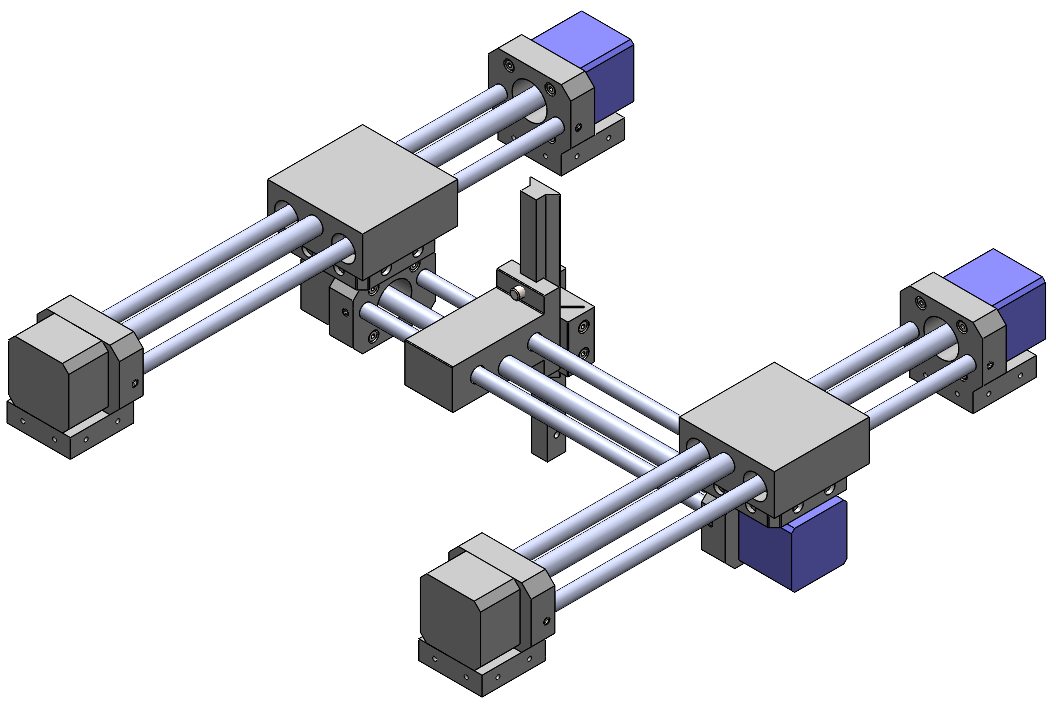
\includegraphics[width=0.8\linewidth]{Sections/6 Detaljeløsning/Media/x,y,z akse.png}
    \caption{Oversigt over x-og y-aksen}
    \label{fig: overview x-y-akse}
\end{figure} 

På billedet kan det ses, at en vogn skal køre frem og tilbage på de to akser. Dette gøres ved at have et gevind inde i vognen, hvor rotationen af ledeskruen vil bevæge vognen frem og tilbage ved \(2\)mm pr. rotation. Der er to følgestænger, som stabiliserer vognen, samt vognen har påsat fire lineære lejre, som mindsker friktion mellem vogn og følgestænger.

Denne konstruktion på henholdsvis x-og y-aksen skal kunne bevæge sig \(200\)mm \(\times\) \(150\)mm, som arbejdsområdet kræver, men har også et krav på tid pr. cm\(^2\), som lyder på 30 sekunder, som begge kan findes i tabel \ref{tab:basale krav}.  Først skal det udregnes, hvor hurtigt robotten kan bevæge sig. Dette kan gøres ved følgende formel:
\begin{equation}
    v=\omega \cdot O
\end{equation}

I formlen for hastigheden er \(\omega\) lig antallet af omdrejninger, som motoren producerer pr. minut, altså 2000 og \(O\) er gevindhældningen på ledeskruen på \(2\)mm. Hastigheden, som ledeskruen kan bevæge sig, er lig \(0,05 \dfrac{m}{s}\).

Dernæst skal tiden fastlægges, både for én bane og dernæst pr. cm\(^2\), hvor én bane er den ene siden af én cm\(^2\), altså \(10\)mm. Der startes med at identificere de faser, som robotten skal igennem, under en bevægelse. Når robotten bevæger sig, skal den igennem tre faser, henholdsvis: Acceleration, bevægelse ved konstant hastighed (top hastighed) og deceleration. Det vil sige, at når tiden skal findes for én bane, kan \(t_{bane}\) defineres som tiden det tager og accelerere og decelerere, samt tiden i top hastighed. Det kan skrives som:
\begin{equation}
\label{Formel:t_{bane}}
    t_{bane}=2 \cdot t_{acc}+t_{top}
\end{equation}

\(t_{bane}\) er defineret udfra, tiden robotten bruger på at accelerere, \(t_{acc}\), samt tiden robotten er i top hastighed, \(t_{top}\). Definitionen af disse to kan findes i bilag \ref{Bilag - Bevægelse} og indsættes på deres respektive pladser i formel \ref{Formel:t_{bane}}:
\begin{equation}
    t_{bane}=2\cdot(\dfrac{m\cdot r^2\cdot \omega}{\tau})+(\dfrac{s_{bane}}{\omega\cdot O}-\dfrac{m\cdot r^2\cdot \omega}{\tau})
\end{equation}
Dette forkortes:
\begin{equation}
    t_{bane}=\dfrac{m\cdot r^2\cdot \omega}{\tau}+\dfrac{s_{bane}}{\omega\cdot O}
\end{equation}

Her er \(m\) lig massen af ledeskruen på \(136\)g. \(r\) er lig radiussen af ledeskruen på \(5\)mm og \(s_{bane}\) er længden af én bane på \(10\)mm. 
Da en cm\(^2\) er defineret som \(10\)mm \(\times\) \(10\)mm, betyder det, at længden af én bane, er lig 10mm. Tykkelsen af en bane er lig \(0,1\)mm, da det er den mindste priktykkelse, som robotten skal kunne placere. Det vil betyde, at \(t_{bane}\) skal ganges med 100, da der skal 100 baner til for at opnå \(1\)cm\(^2\):
\begin{equation}
    t_{cm^2}=t_{bane}\times 100
\end{equation}

Tiden pr. cm\(^2\) er lig \(15,1\)s, hvilket betyder, at kravet om tidsforbrug pr. cm\(^2\) på 30 sekunder er opfyldt og at robotten bevæger sig, som den skal i x-og y-retningen. Den fulde formeludledning med symboler kan findes i bilag \ref{Bilag - Bevægelse}.
\end{comment}


\plainbreak{2}
\subsection{Orientering af følgestænger}\label{afs: Orientering af stænger}

%Præcision under accelererende bevægelse kan observeres ved at kigge på den kraft der går igennem massen på stængerne under acceleration eller deceleration. Fra designspecifikation 3 må prikplacering ikke variere mere end $0,1$mm. Udbøjningen i x-aksen må derfor ikke overstige $0,1$mm. idet afstanden fra PeJV til bundpladen vil variere og ændre prikstørrelsen. Da det er de samme stænger med samme randbetingelser kan den samme formel for udbøjning bruges, med kraften der kommer fra accelerationen. Derudover er de to følgestænger side om side bedre til at modstå udbøjning i xy-planet, da der i dette plan vil være flytningsbidrag imellem de to følgestænger. Forskellen kan ses på figur \ref{fig: Flytningsbidrag1} og \ref{fig: Flytningsbidrag2}

Før der kan beregnes den belastning, som følgestængerne udsættes for, er det nødvendigt at fastlægge deres optimale orientering i forhold til ledeskruen. Orienteringen har direkte indflydelse på stellets samlede udbøjning og da kravet til præcisionen på prikplaceringen er maks. $\SI{\pm0,1}{mm}$ (præstationskrav 3), må udbøjningen aldrig overstige denne grænse. 

Der vurderes at der er to mulige placeringer, henholdsvis følgestængerne placeret vertikalt over hinanden eller horisontalt ved siden af hinanden, som vist i figur \ref{fig: Flytningsbidrag1} og \ref{fig: Flytningsbidrag2}.

\begin{figure}[H]
    \centering
    \begin{subfigure}[b]{0.45\textwidth}
    \centering
        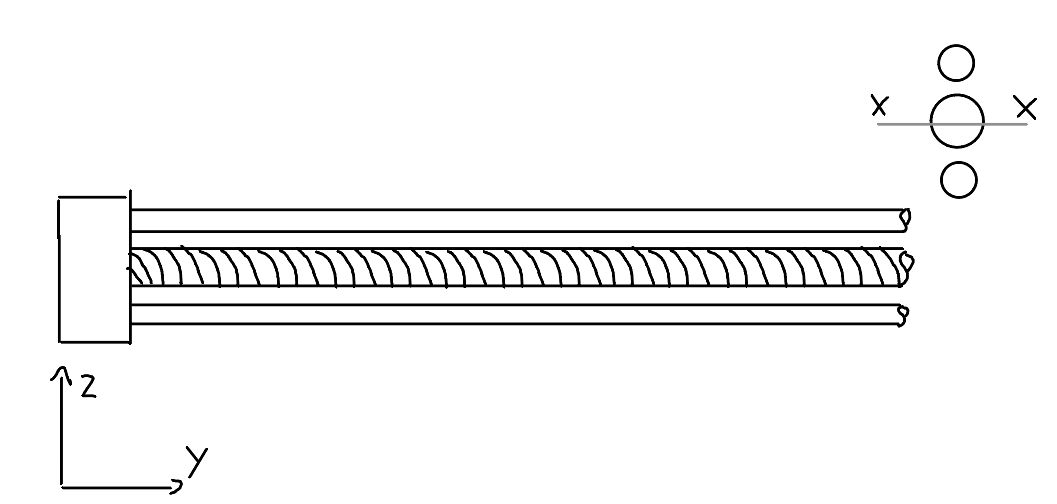
\includegraphics[width=\textwidth]{Sections/6 Detaljeløsning/Media/Tværsnit x-x.png}
        \caption{Tværsnit når følgestængerne er over hinanden} 
        \label{fig: Flytningsbidrag1}
    \end{subfigure}
    \hfil
    \begin{subfigure}[b]{0.5\textwidth}
    \centering
        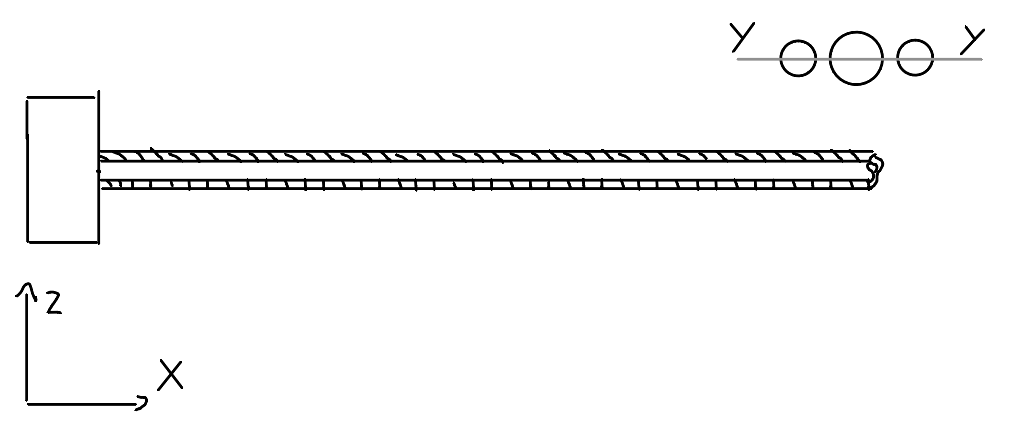
\includegraphics[width=0.9\textwidth]{Sections/6 Detaljeløsning/Media/Tværsnit y-y.png}
        \caption{Tværsnit når følgestængerne er ved siden af hinanden} 
        \label{fig: Flytningsbidrag2}
    \end{subfigure}
    \caption{Følgestængers placering i forhold til ledeskruen}
\end{figure}

Herfra ses der på hvilke kræfter som de lineære akser bliver udsat for. Aksernes egen masse samt punkmassen af PeJV'en vil vil have en lodret nedad rettet kraft. Derudover er der en kraft fra accelerationen og deaccelerationen af de lineære akser. Det vides at den nedadrettetede acceleration er tyngdeaccelerationen på $\SI{9,82}{m/s^2}$ og fra afsnit \ref{Kinematisk analyse} vides det at den lineære acceleration er på $\SI{70,8}{m/s^2}$. Dette betyder at det er denne laterale kraft som følgestængerne skal orienteres efter, da denne er størst. Derved skal følgestængerne være i den horisontale position for at modvirke bøjningen bedst og derved have den bedst mulige præcision. Flytningsbidraget afhænger af afstandsforskellen i bøjningsretningen i anden, i forhold til positionen af stængerne. Derfor afhænger flytningsbidraget af afstanden imellem stængerne i anden. 
\begin{figure} [H]
    \centering
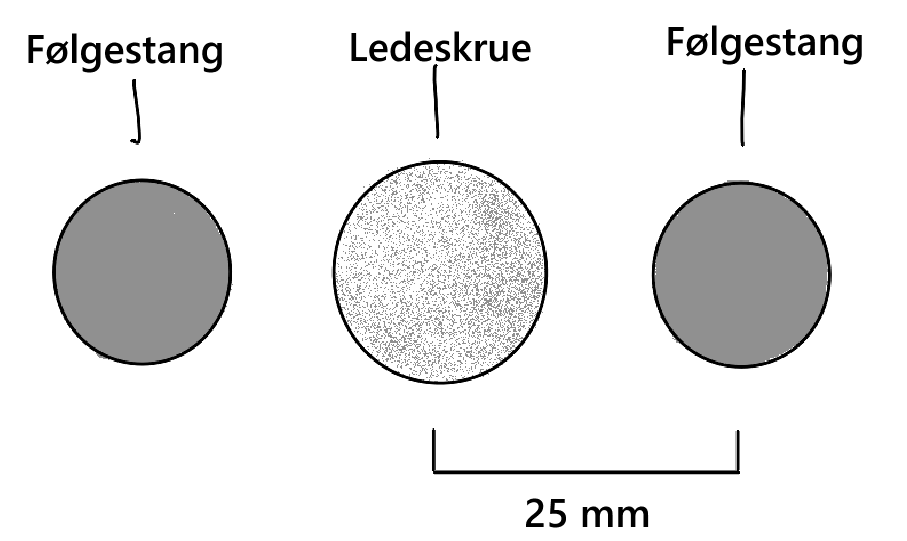
\includegraphics[width=0.5\linewidth]{Sections/6 Detaljeløsning/Media/Ledeskrue-afstand.png}
    \caption{Tværsnit af ledeskrue og følgestanger med indtegnet flytningsbidrag}
    \label{fig:flytningsbidrag}
\end{figure}
For at give et betydeligt flytningsbidrag, er der valgt en afstand på $\SI{25}{mm}$ fra ledeskruens centrum, til følgestængernes centrum, se figur \ref{fig:flytningsbidrag}. Dette giver også plads til følgestængerne og ledeskruen, så de ikke rører hinanden.




\plainbreak{2}
\subsection{Vertikal udbøjning af ledeskrue} \label{Præcisions beregninger}
Designspecifikation 3 angiver at placeringen af en prik ikke må afvige mere end \(\SI{\pm0,1}{mm}\) fra punktet hvor prikken er angivet af softwaren. Denne præcision afhænger af motorens præcision, tolerancerne imellem ledeskruen og vognen, samt udbøjning af materialet ($W(y)$). Hvis stellet og bevægelsesdelene ikke har en tilstrækkelig stivhed vil der ske udbøjning, som resulterer i, en afvigelse af prikplaceringen. Det vælges at hovedet skal bevæges i alle 3 akser, fordi det vurderes at veje mindre end bundpladen og emnet. Dette giver mindre masse der skal flyttes, hvorved højere præcision kan opnås. Udbøjningen af den lineære y-akse i z-retningen kan bestemmes ved formel \ref{formel: udbøjning}.
\begin{equation} \label{formel: udbøjning}
    W(y)=\iint \frac{M(y)}{E \cdot I} dy^2
\end{equation}
\begin{figure}[H]
    \centering
    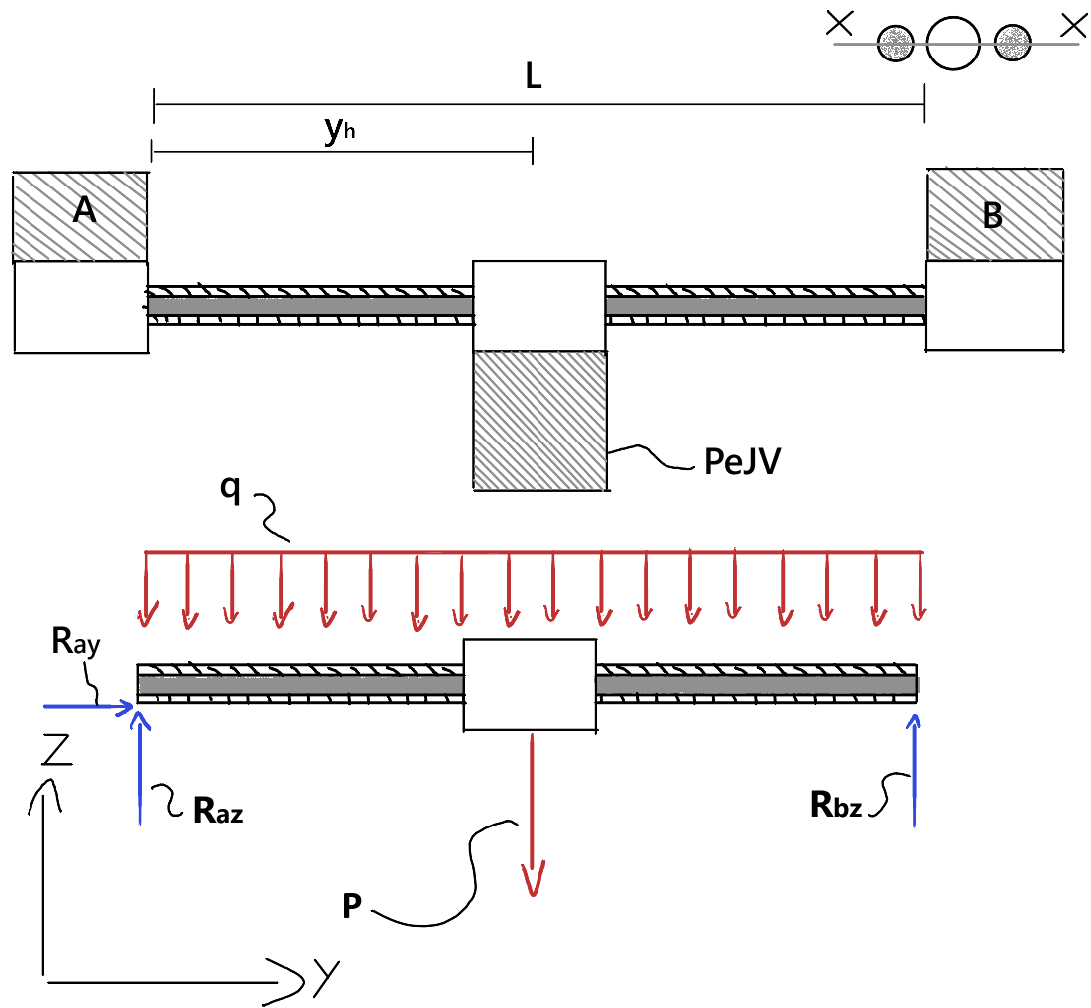
\includegraphics[width=0.6\linewidth]{Sections/6 Detaljeløsning/Media/FLD - y-akse.png}
    \caption{Fritlegeme diagram over y-aksen}
    \label{fig: FLD y-udbøj}
\end{figure}

Momentligningen ($M_{max}(y)$) er udledt fra bilag \ref{bilag- statik udledning} i formel \ref{formel: M_max(y)}. Denne formel er udledt af betingelserne fra figur \ref{fig: FLD y-udbøj}, hvor P's placering er uafhængig på stængerne. Ligningen for momentet indsættes i udbøjningsligningen \ref{formel: udbøjning}.
\begin{equation}
    W(y)=\iint \frac{P\cdot \left(y-\frac{y^2}{L}\right)+\frac {q\cdot L}{2}\cdot\left( y-\frac{y^2}{L}\right)}{EI}dy^2
\end{equation}

Herefter dobbeltintegreres med hensyn til y:
\begin{equation} \label{formel: W_y med M og I}
   W(y)= \frac{P\cdot \left(\frac{y^3}{6}-\frac{y^4}{12\cdot L}\right)+\frac {q\cdot L}{2}\cdot\left(\frac{y^3}{6}-\frac{y^4}{12\cdot L}\right)}{EI} + C_1 y+C_2
\end{equation}

Da det er en simpel understøtning i begge ender af stængerne, indebærer det, at der ikke kan være en udbøjning i enderne. Dette giver randbetingelserne $W(0)=0$ og $W(L)=0$, der bruges til at finde konstanterne i \ref{formel: W_y med M og I}.
\begin{equation} \label{formel: W(0)}
        W(0)= \frac{P\cdot \left(\frac{0}{6}-\frac{0}{12\cdot L}\right)+\frac {q\cdot L}{2}\cdot\left(\frac{0}{6}-\frac{0}{12\cdot L}\right)}{EI} + C_1 0+C_2=0
\end{equation}

Når $y=0$ kræver det at $C_2=0$ for at opfylde kriteriet.
\begin{equation} \label{formel: W(L)}
       W(L)=\frac{P\cdot \left(\frac{L^3}{6}-\frac{L^4}{12\cdot L}\right)+\frac {q\cdot L}{2}\cdot\left(\frac{L^3}{6}-\frac{L^4}{12\cdot L}\right) }{EI} + C_1\cdot L=0
\end{equation} 

Ved $y=L$ fås $C_1=-\frac{P\cdot L^2}{12\cdot EI}-\frac{q\cdot L^3}{24\cdot EI}$. Disse konstanter indsættes i formel \ref{formel: W_y med M og I} for at få et endeligt udtryk for udbøjningen af stængerne.
\begin{equation} \label{formel: W(y) med C1 og C2}
   W(y)= \frac{P\cdot \left(\frac{y^3}{6}-\frac{y^4}{12\cdot L}-\frac{L^2\cdot y}{12}\right)+\frac {q\cdot L}{2}\cdot\left(\frac{y^3}{6}-\frac{y^4}{12\cdot L}-\frac{L^2\cdot y}{12}\right)}{E\cdot\frac{\pi}{2}\cdot r_f^4}
\end{equation}

For at holde præcisionen og farten i ledeskruen, er det nødvendigt at skruen ikke udbøjer mere end \(\SI{\pm0,1}{mm}\). Det er vurderet da en stor udbøjning resulterer i et spænd af skruen og følgestængerne. Det vælges at benytte følgestænger lavet i 1060 Carbon stål met et E-modul på omkring 200 GPa. For at undersøge sammenhængen imellem radius af følgestængerne og udbøjningen, plottes formel \ref{formel: W(y) med C1 og C2}. I denne formel og på dette plot, vil den maksimale udbøjning vurderes i forhold til radius af følgestængerne. Dette plot bruges til at finde, hvad radius skal være for at undgå \(\SI{\pm0,1}{mm}\) udbøjning.

\begin{figure}[H]
    \centering
    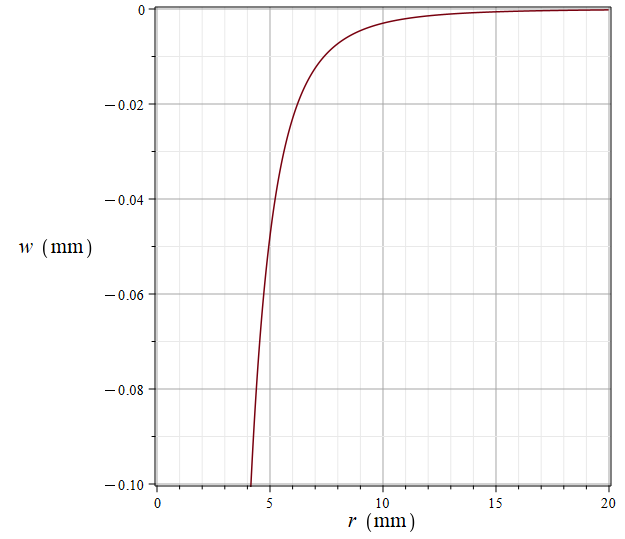
\includegraphics[width=0.5\linewidth]{Sections/6 Detaljeløsning/Media/Udbøjning ifht. r.png}
    \caption{Kurve for udbøjning på x-aksen, afhængigt af radius på følgestænger.}
    \label{fig: Udbøjninggraf}
\end{figure} \plainbreak{-0.5}

Af figur \ref{fig: Udbøjninggraf} fremgår det, at en radius på lidt over $\SI{4}{mm}$, vil opfylde kravet om mindre end $\SI{\pm 0,1}{mm}$ udbøjning. Under antagelserne, der er lavet omkring punktlastens placering, vurderes det at det værste tilfælde i forhold til udbøjning forekommer, når hovedet af prikværktøjet er så tæt på den ene af de lineære x-akser som muligt. Her vil kun ét af de to lineære x-akser bære hele hovedets vægt. Dette kan ikke lade sig gøre i virkeligheden, da hovedets dimensioner vil holde det fra, at være placeret lige under stængerne for den lineære x-akse. Dermed vil der i virkeligheden, altid være noget af vægten der holdes af stængerne på den anden side, hvilket betyder at det faktiske værste tilfælde er mindre udbøjet end der vises i formlen. Dette kan ses på figur \ref{fig: Udbøjningpraktik}.

\begin{figure}[H]
    \centering
    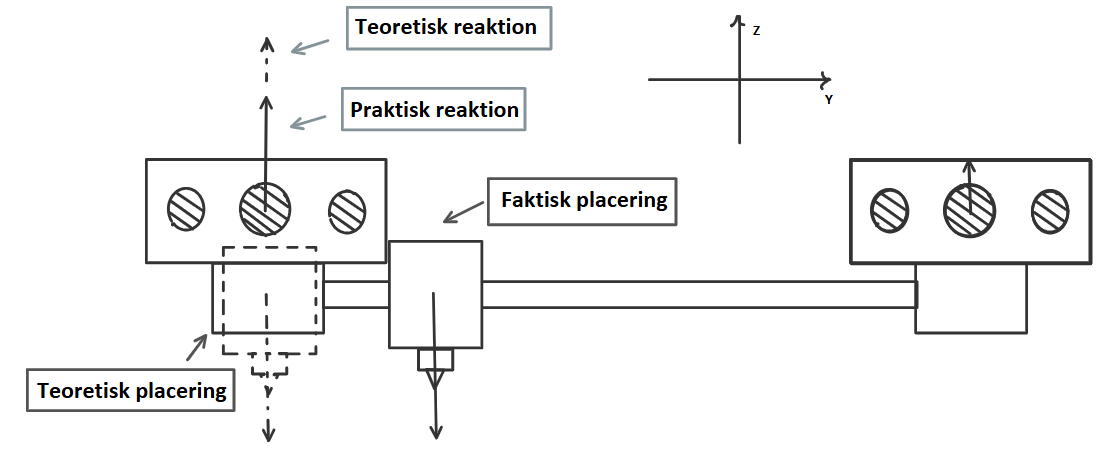
\includegraphics[width=0.8\linewidth]{Sections/6 Detaljeløsning/Media/Praktisk vs teoretisk udbøjning.png}
    \caption{Skitse af den teoretiske reaktion og den praktiske reaktion af de lineære x-akser}
    \label{fig: Udbøjningpraktik}
\end{figure}

Dette betyder, at udregninger giver en sikkerhedsfaktor i forhold til virkelighedens udbøjning. Derudover er det også antaget, at ledeskruen ikke vil bære noget vægt, og i virkeligheden vil det ikke være muligt, og derfor vil den faktiske udbøjning også skulle bøje ledeskruen, som har en diameter på $\SI{10}{mm}$. Dette er også en sikkerhedsfaktor, og derfor vurderes kravet i forhold til maksimal udbøjning opfyldt.


\plainbreak{2}
\subsection{Udbøjning i xy-planet af ledeskrue}
I afsnit \ref{afs: Orientering af stænger} blev det klargjort at den største acceleration findes vinkelret på stængerne i xy-planet, når hovedet accelererer. Hovedets acceleration vil skabe en kraft grundet hovedets masse. Her vil flytningsbidraget være med til at modarbejde udbøjningen som nævnt i afsnit \ref{afs: Orientering af stænger}. Udbøjningen for stængerne i xy-planet, som resultat af disse kræfter udregnes. Dette gøres, for teoretisk at finde ud om løsningen lever op til præstationskrav 3. Formlen \ref{formel: I_xx med x^2 og A} angiver inertimomentet om z-aksen med flytningsbidraget. 
\begin{equation} \label{formel: I_xx med x^2 og A}
    I_{zz}=I_{zz1}+z^2\cdot A
\end{equation}

Her er $I_{zz}$ det samlede inertimoment, $I_{zz1}$ er inertimomentet uden flytningsbidrag, $z^2$ er højdeforskellen imellem arealmidtpunktet og hvert dels arealmidtpunkt og A er arealet af hver del. I dette tilfælde udbøjes om z-aksen i stedet for x- eller y-aksen, hvilket betyder flytningsbidraget afhænger af længde/bredde forskellen i anden fra arealmidtpunktet. Forskellen i bredde/længde af følgestængerne er \(\SI{50}{mm}\). Da de er lige store vil arealmidtpunktet være placeret med lige stor afstand i mellem dem og midten, altså \(\SI{25}{mm}\). Arealet er cirkulært og skrives derfor som $\pi \cdot r_f^2$.
\begin{equation}
    I_{zz}=I_{zz1}+y^2\cdot \pi\cdot r^2_f
\end{equation}

Kraften der påvirker udbøjningen vil være massen af hovedet ganget med dets acceleration. Denne kraft er fundet fra formel \ref{formel: Accelerationskraft}, og kan bruges igen i dette tilfælde. Udbøjningsligningen vil genbruges fra tidligere afsnit, da randbetingelserne og vilkårene er de samme i forhold til kraftens placering. I dette tilfælde skal inertimomentet og kraften opdateres til de nye værdier nævnt i dette afsnit.




\section{Opsummering på nøjagtgihed af prikplacering}


\renewcommand{\arraystretch}{1.3}
\begin{table}[H]
\setlength{\tabcolsep}{20pt}
 \centering
  \caption{Variabelliste}
 \begin{tabular}{|l c c|} \hline

  \multicolumn{3}{|c|}{\cellcolor{aaublue} \color{white} \textbf{NEMA 14 motor}}  \\\hline
 \rowcolor{gray!10}  \multicolumn{1}{|c}{\textbf{Beskrivelse}} & \multicolumn{1}{c}{\textbf{Symbol}}  & \multicolumn{1}{c|}{\textbf{Værdi}}  \\\hline
 Drejningsmoment af motor & \(\tau\) &\SI{0,12}{Nm}\\\hline
 Vinkelhastighed af motor & \(\omega\) & \SI{2000}{RPM}\\\hline
 Præcision af ledeskruen & \(\delta\) & \SI{0,01}{mm}\\\hline
 \specialrule{1pt}{0pt}{0pt}
 
  \multicolumn{3}{|c|}{\cellcolor{aaublue} \color{white} \textbf{Kinematik og statik}}  \\\hline
 \rowcolor{gray!10} \multicolumn{1}{|c}{\textbf{Beskrivelse}} & \multicolumn{1}{c}{\textbf{Symbol}} & \multicolumn{1}{c|}{\textbf{Værdi}}  \\\hline
  Tid pr. $\SI{}{cm^2}$ & \(t_{cm^2}\) & \SI{15,1}{s}\\\hline
  Acceleration & \(a\) & \SI{70,8}{m/s^2}\\\hline
  Radius af ledeskrue & \(r_l\) & \SI{5}{mm}\\\hline
  Gevindhældning af ledeskrue & \(O_l\) & \SI{2}{mm}\\\hline
  Radius af følgestænger & \(r_f\) & \SI{4}{mm}\\\hline
  Maksimal udbøjning & $W(y)_{max}$ & \SI{6,5d-3}{mm}\\\hline

 \end{tabular}
 \label{tab: variabelliste}
\end{table}

Udbøjningen kommer til at være maksimalt $\SI{6,5d-3}{mm}$, og er dermed under kravet om $\SI{\pm0,1}{mm}$ afvigelse. Summen af tolerancerne fra udbøjningen og steppet i motoren må angive den samlede tolerance i forhold til præcision af prikplacering. Summen bliver $\SI{6,5d-3}{mm}+\SI{d-2}{mm}$ = $\SI{16,5d-3}{mm}$, hvilket er under afvigelsen på  $\SI{\pm0,1}{mm}$ med en faktor 6. Kravet om prikpositionspræcision er derved opfyldt.


\begin{comment}
Præcision under accelererende bevægelse kan observeres ved at kigge på den kraft der går igennem massen på stængerne under acceleration og deceleration. Fra designspecifikation 3 må prikplacering ikke variere mere end $0,1$mm. Udbøjningen i x-aksen må derfor ikke overstige $0,1$mm, idet afstanden fra PeJV til bundpladen vil variere og ændre prikstørrelsen. Da det er de samme stænger med samme randbetingelser kan den samme formel for udbøjning bruges, med kraften der kommer fra accelerationen. Derudover er de to følgestænger side om side bedre til at modstå udbøjning i xy-planet, da der i dette plan vil være flytningsbidrag imellem de to cylindre. Forskellen kan ses på figur \ref{fig: Flytningsbidrag1} og \ref{fig: Flytningsbidrag2}
\begin{figure}[H]
    \centering
    \begin{subfigure}[b]{0.4\textwidth}
        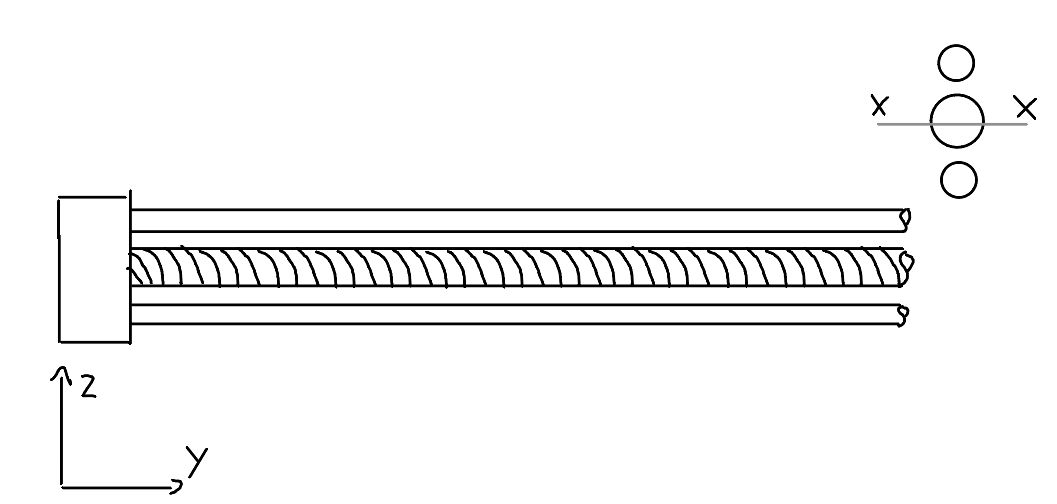
\includegraphics[width=\textwidth]{Sections/6 Detaljeløsning/Media/Tværsnit x-x.png}
        \caption{Tværsnit når følgestængerne er over hinanden} 
        \label{fig: Flytningsbidrag1}
    \end{subfigure}
    \begin{subfigure}[b]{0.52\textwidth}
        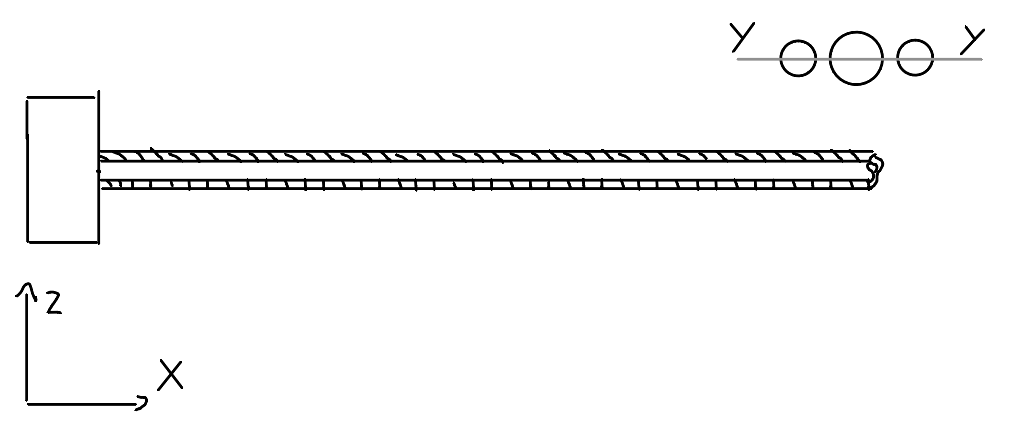
\includegraphics[width=\textwidth]{Sections/6 Detaljeløsning/Media/Tværsnit y-y.png}
        \caption{Tværsnit når følgestængerne er ved siden af hinanden} 
        \label{fig: Flytningsbidrag2}
    \end{subfigure}
    \caption{Følgestængers placering i forhold til ledeskruen}
\end{figure}

Med flytningsbidrag hedder inertimomentet følgende
\begin{equation} \label{formel: I_xx med x^2 og A}
    I_{xx\perp}=I_{xx}+z^2\cdot A
\end{equation}
Det nye inertimoment findes altså ved at tage det gamle og lægge et flytningsbidrag til. Flytningsbidraget findes ved at gange højden i anden på forskellen fra areamidtpunktet med arealet. Arealet af en cylinder findes ved formlen $\pi\cdot r^2$ og kan indsættes på A's plads. Derudover er konstruktionen lavet med $50$mm i mellem de to cylindre, og der vil derfor være $25$mm til arealmidtpunktet for begge cylindre.
\begin{equation}
    I_{xx}=I_{xx1}+z^2\cdot \pi\cdot r^2
\end{equation}
For at kende udbøjningen er det nødvendigt at finde kraften der påvirker stængerne. Her bruges Newtons anden lov $F=m\cdot a$, hvor massen er massen af lasten der sidder på stængerne og accelerationen er skruens egenskab til at bremse/accelerere lasten. I bilag \ref{Bilag - Bevægelse} ses det, at den lineære acceleration kan skrives som $a=\alpha \cdot O$, hvor O er gevindhældningen i skruen og alpha er vinkelaccelerationen. Vinkelaccelerationen kan omskrives i dette tilfælde også fra bilag \ref{Bilag - Bevægelse} til $\frac{\tau}{m\cdot r^2} $. Dermed må kraften kunne skrives som:
\begin{equation}
    F=\frac{m_v\cdot O\cdot \tau}{m_l\cdot r_l^2} 
\end{equation}
Hvor $m_v$ er massen af lasten, $\tau$ er momentet fra motoren, $m_l$ er massen af ledeskruen og $r_l$ er radius af ledeskruen. Når denne kraft, og det fundne inertimoment indsættes kan den nye udbøjning findes, og den maksimale udbøjning bliver $8\mu m$ og er dermed inden for $0,05mm$ tolerance i forhold til præcision.    
\end{comment}




\plainbreak{2}
\section{Løsningens design} \label{Dimensionering af stellet}

Designet af de lineære bevægelser og stellet der understøtter dem beskrives i dette afsnit. Her tages udgangspunkt i opfyldelse af følgende præstationskrav. 

\begin{itemize}
    \item[4.] Størrelse på arbejdsområde på over \SI{200}{mm} $\times$ \SI{150}{mm} $\times$ \SI{50}{mm} 
    \item[11.] Mængde af forskellige værktøjer til samling på 5 stk.
    \item[12.] Mængde af specialværktøj til samling af robot på maksimum 1 stk.
\end{itemize}

Stellet udformes, så arbejdsområdet er over \SI{200}{mm} $\times$ \SI{150}{mm} $\times$ \SI{50}{mm}, med hensyn til følgestænger og ledeskruens diameter. 




%Stellet laves af 40mm \(\times\) 40mm aluminiums t-slots profiler. Dette er med til at gøre motoren mere stabil, så ledeskruen holdes mere stabil, og derigennem kommer mindre afvigelser i præcision under bevægelse.

%Dette er med til at holde sig inden for designspecifikation 3, som kræver en tolerance på under 0,05mm. 

%Fordi der bruges en ledeskrue til bevægelsen, skal der være følgestænger/guide stænger til at tage lasten, så ledskruen ikke udbøjer. Dette giver en højere præcision, fordi grænseværdien i designspecifikation 3 for variation på prikplacering er 0,05mm, hvilket oversættes til, at udbøjningen heller ikke må overstige denne værdi i xy-planet. Det er derfor nødvendigt at kigge på udbøjningen som konsekvens af ladet på stangens acceleration under påføring af speckle pattern. Derudover er det vigtigt at motoren og ledeskruen kan holde den samme tolerance og fart under prikpåføring og bevægelse. Det er derfor relevant at motoren og skruens frekvens ikke er forstyrret, samt at skruens bøjning ikke forstyrrer overførslen af rotation til lineær bevægelse. For at sikre dette, optimeres følgestængerne til at have en udbøjning under 0,1mm, for at mindske effekten af udbøjningen på arbejdet af skruen og motoren. 

%For at opnå den ønskede specifikation på arbejdsområdet, på $200mm\times150mm\times50mm$ fra præstationskrav 4, udformes pladen arbejdsområdet består, med plads til indspænding, hvilket opnås ved at tilføje 35mm mere i hver side. Dette giver plads, til at prikværktøjet kan nå kanterne af arbejdsområdet, da vognen der kører på ledeskruen, har en bredde der gør, at der skal ekstra plads til at hovedet kan placeres over kanten af arbejdsområdet. 

%I den ene ende af stængerne vil der være en motor monteret, som skal sørge for at ledeskruen og derigennem prikværktøjet bliver flyttet i den ønskede retning. Derudover ved motoren vil der være en indspænding til følgestængerne. Motoren er spændt fast til indspændingen og indspændingen er spændt fast til stellet. I den anden ende af ledeskruen sidder der en indspændingsklods, som modtager og fastlåser positionen af ledeskruen og de to følgestænger. Positionen af indspændingsklodsen er fastlåst til stellet, og derigennem er skruen og følgestængernes placering låst til stellet. Dette gør flytningerne langs med skruen minimale, og sørger for, at skruen er stabil, således præcision og fart kan vedligeholdes under bevægelse.

%For at opfylde designspecifikation 4, der kræver dimensioner på arbejdsområdet til $200mm\times150mm\times50mm$. Dette betyder at det skal være muligt at prikke emner inden for disse grænser. For at gøre dette er det nødvendigt at kunne ændre højden af hovedet for at nå en afstand til emnet, hvor prikværktøjet er præcist. Derfor er prikværktøjet indspændt med et dovetailled, som kan løsnes og fastnes med en skrue. Når denne skrue er løsnet er det muligt at bevæge prikværktøjet op og ned med tilstrækkelig præcision, for at afstanden imellem prikværktøjet og prikoverfladen er tilstrækkelig til speckle pattern påføring.

%Designspecifikation 8 kræver et tidsforbrug under 30 sekunder pr. cm${^2}$ til prikplacering. Prikværktøjet er lavet til at kunne prikke i bevægelse, derfor kan den gå fra den ene ende af kvadratcentimeteren til den anden inden den skal bremse. Dette betyder at den skal accelerere og decelerere én gang per bane. De tyndeste prikker der kan laves er 0,1mm, og der vil derfor for at dække hele kvadratcentimeteren skulle 100 baner af 0,1 mm langs de 10 mm for at kunne dække hele kvadratcentimeteren med prikker. Det betyder 100 accelerationer og decelerationer pr. kvadratcentimeter. Der kan altså skrues på en motors topfart og accelerationsevne for at nå dette mål.

%For y-aksens ledeskrue og følgestængerne ikke udbøjer og derved mindsker præcisionen, er de spændt fast i en indspænding, som er monteret til en vogn på den parallelt liggende ledeskrue. Denne indspændingen er udformet så dens vægt tilnærmer sig vægten fra motoren, dette valg med at lave en kontravægt er for at udbøjningen og bevægelsen på de to sæt følgestænger på x-aksen, er så ens som muligt. Denne ens bevægelse er nødvenlig for opretholde den påkrævet præcision, da uens bevægelse vil kunne medføre ledskruen på y-aksen står skævt og derved give fejlplacering i xy-planet. 
\subsection{Valg af standard komponenter} \label{Standard komponenter}
Stellet laves af standard komponenter, for at opfylde præstations krav 11 og 12 om antal værktøj der skal benyttes til at samle robotten, samt minimere omkostninger til produktion af enkelt komponenter. Der gøres brug af $\SI{40}{mm}\times\SI{40}{mm}$ aluminiums t-slots profiler, som ses i figur \ref{fig:T-slot profil 1}. T-slot profiler (også kendt som aluminiumsprofilrammer) er kendetegnet ved de åbne T-formede spor langs deres sider, som tillader ned og fleksible montering af beslag, skruer og andre komponenter. Dette gør dem særligt velegnet til maskinstel, arbejdsstationer og robotsystemer, hvor modularitet og præcision ønskes. Aluminium T-slot profilrør leveres i standard størreler, hvortil diverse standard T-slots beslag og notsten kan tilkøbes. \parencite{McMaster-Carr2025T-slottedFraming}

\begin{figure}[H]
    \centering
    \begin{subfigure}[b]{0.34\textwidth}
        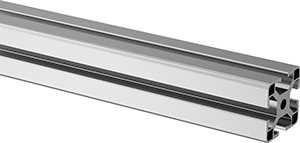
\includegraphics[width=\textwidth]{Sections/6 Detaljeløsning/Media/T-slots.png}
        \caption{Alu T-slot profilrør.} 
        \label{fig:T-slot profil 1}
    \end{subfigure}
    \hfill
    \begin{subfigure}[b]{0.4\textwidth}
       \centering
        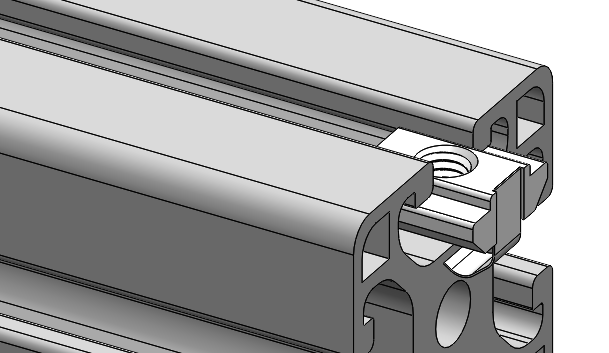
\includegraphics[width=.9\textwidth]{Sections/6 Detaljeløsning/Media/T-slot med Notsten.png}
        \caption{Alu T-slot profilrør med notsten} 
        \label{fig: T-slot profil med notsten}
    \end{subfigure}
     \hfill
    \begin{subfigure}[b]{0.24\textwidth}
        \centering
        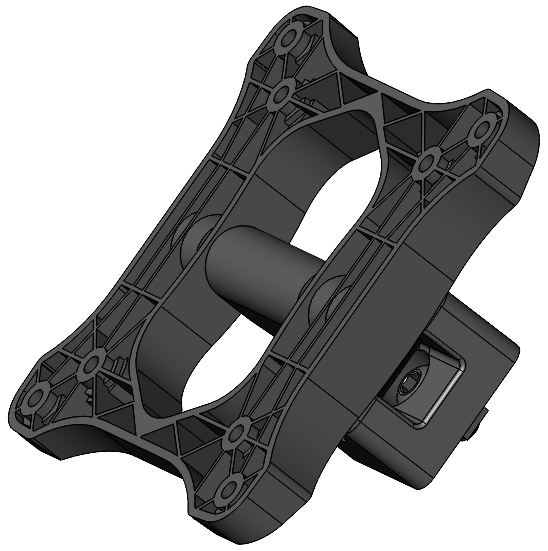
\includegraphics[width=.9\textwidth]{Sections/6 Detaljeløsning/Media/kontrolsystem montage1.png}
         \caption{Monterings element}
    \label{fig:T-slot tablet holder}
    \end{subfigure}
    \caption{T-slot profil rør med notsten og monterings element. \textit{(c)} er til montering af elektronik efter VESA (Video Electronics Standards Association) til standard i T-slot alu profilrør. Billeder fra \parencite{McMaster-Carr2025T-SlottedRails}}
\end{figure} \plainbreak{-1}

Aluminium T-slot profilrør gør det muligt, at montere kontrolsystemet alle steder på stellet, hvor der ikke er beslag. Montage sker ved at indsætte notsten i t-slotten, som set på figur \ref{fig: T-slot profil med notsten}, hvor bolte kan skrues i. Kamera og skærm kan for eksempel monteres ved brug af monterings elementer, som det der kan ses i figur \ref{fig:T-slot tablet holder}. \parencite{McMaster-Carr2025T-slottedFraming}.





%I konstruktionen af stellet er der brugt t-slot aluminiumsrammer. Til påsætning er det derfor muligt, at montere midler med t-slot ender på stellet. Denne monteringsmetode gør det muligt at sætte mange forskellige monteringsmidler til forskellige kameraer og skærme, til kontrolsystemets opgaver.
\begin{comment}
    \begin{figure}[H]
    \centering
    \begin{subfigure}[b]{0.48\textwidth}
        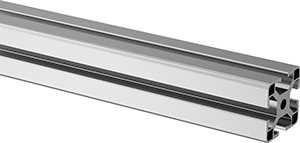
\includegraphics[width=\textwidth]{Sections/6 Detaljeløsning/Media/T-slots.png}
        \caption{Alu T-slot profilrør. \parencite{McMaster-Carr2025T-SlottedRails}} 
       
    \end{subfigure}
    \hfill
    \begin{subfigure}[b]{0.48\textwidth}
    \centering
        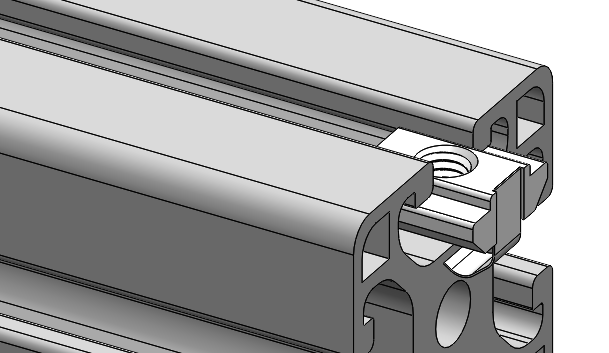
\includegraphics[width=.9\textwidth]{Sections/6 Detaljeløsning/Media/T-slot med Notsten.png}
        \caption{Alu T-slot profilrør med notsten} 
        
    \end{subfigure}
    \caption{}
\end{figure} \plainbreak{-1}


\begin{figure}[H]
    \centering
    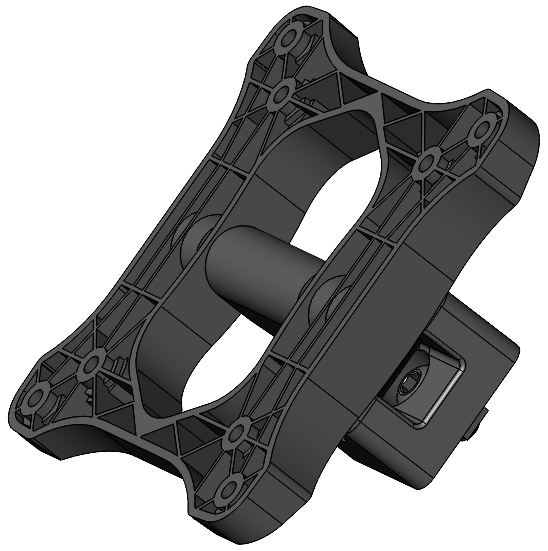
\includegraphics[width=0.3
    \linewidth]{Sections/6 Detaljeløsning/Media/kontrolsystem montage1.png}
    \caption{Montering af elektronik efter VESA (Video Electronics Standards Association) standard i T-slot alu profilrør }
    
\end{figure} \plainbreak{-1}
\end{comment}

\plainbreak{2}
\subsection{Design af Lineær bevægelse i x-, y- og z-retningen} \label{Design af Lineær bevægelse i x-, y- og z-retningen}

Det er valgt at bevæge de to akser seperat, hvilket sikrer at det ønskede arbejdesområde kan tilgås præcist. Arbejdsområdets ene side er længere end den anden, og afstanden har indflydelse på udbøjningen. Det vælges derfor at doserings mekanismen monteres på den korte akse, y-aksen, dette er gjort for at minimere udbøjningen, som det ses i afsnit \ref{Præcisions beregninger}.

Som tidligere beskrevet bevæges y-aksen og hovedet med ledeskruer på $\diameter\SI{10}{mm}$, både x og y vognen glider på to følgestænger, placeret horisontal på hver side af ledeskruen. Hver ledeskrue drives af en NEMA 14 motor, som det ses på figur \ref{fig:xyz akse med navne}. Følgestængerne bære vægten af henholdsvis x-vognen og y-vognen, gennem glidelejre for at minimere friktion. I den modsatte side af motoren er ledeskruen drejet rund og monteret i et kugleleje.


\begin{figure}[H]
    \centering
    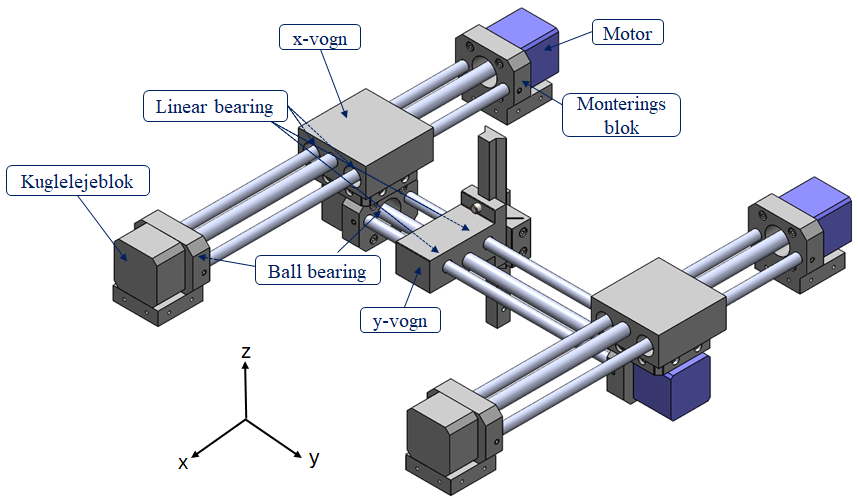
\includegraphics[width=0.8\linewidth]{Sections/6 Detaljeløsning/Media/x,y,z akse med tekst.png}
    \caption{x-, y- og z-aksen med navne}
    \label{fig:xyz akse med navne}
\end{figure} \plainbreak{-0.5}
 
Det er valgt, at y-aksen er fastspændt under x-aksen, så der kan påsættes prikker på emner under \(\SI{50}{mm}\), med den valgte justering af z-aksen. Robotten skal kun håndtere objekter med plane flader, hvorfra det ikke er nødvendigt, at justere z-aksen under processen. Det vælges derfor, at z-aksen justeres manuelt inden robotten startes. Dette gøres med en svanehalemekanisme på y-vognen, som ses i figur \ref{fig:z-akse justering}.

\begin{figure}[H]
    \centering
    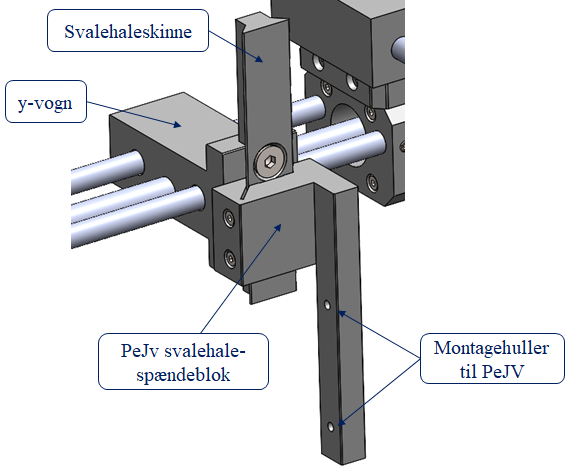
\includegraphics[width=0.6\linewidth]{Sections/6 Detaljeløsning/Media/z-akse med tekst.png}
    \caption{y-vogn med svalehaleblok og svalehale skinne, der bruges til justering af z-aksen. Jet valve DV-6210 monteres på svalehaleskinnen med to M4 bolte i montagehullerne.}
    \label{fig:z-akse justering}
\end{figure} \plainbreak{-0.5}

Her monteres Jet Valve DV-6210 med to M4 bolte i montagehullerne. Svalehaleblokken sættes på y-vognen, hvorefter svalehaleskinnen frit kan bevæges fra bundpladen \(\SI{60}{mm}\) over bundpladen. Alle komponenterne til den lineære bevægelse, der er designet til løsningen, produceres i Aluminium EN AW-6082 T6.

Aluminium EN AW-6082 T6 er et let metal med en densitet på cirka \(\SI{2700}{kg/m^3}\) og et E-modul omkring \SI{71}{GPa}. Aluminiumet tilbyder et gunstigt forhold mellem vægt og stivhed, hvilket gør det velegnet til strukturer, hvor lav masse og tilstrækkelig mekanisk styrke er væsentlige krav. Materialets flydespænding er \SI{255}{MPa}, og dets trækstyrke spænder fra \SI{300}{MPa} til \SI{340}{MPa}. EN AW-6082 T6 har desuden gode bearbejdningsegenskaber, idet det let kan fræses, bores og svejses. En yderligere fordel er dets naturlige korrosionsbestandighed, hvilket reducerer behovet for omfattende overfladebehandling i mange anvendelser. Aluminium er samtidig relativt økonomisk tilgængeligt med en gennemsnitlig pris på omkring 244 DKK pr. kg \parencite{Aluminiumplade}. Ulempen ved aluminium er dog, at materialet i visse tilfælde kan have begrænset modstandskraft over for høje punktbelastninger, hvilket kan føre til lokal plastisk deformation, hvis konstruktionen ikke dimensioneres tilstrækkeligt. \parencite{Hesse2011AluminiumSheets}.


%Da der arbejdes med emner der har en ens højde langs hele emnet, betyder det at under processen behøver der ikke sker regulering i z-aksen. Det er derved blevet valgt at bevægelsen på z-aksen, sker manuelt inden processen starter. 

%De to resterende akser udspænder det planen som der skal kunne sættes prikker. 

%Bevægelsen i xy-planet kommer derved fra to ledskruer på x-aksen og en ledeskrue på y-aksen. Ledeskruerne på x-aksen driver hver deres vogn, som hvorpå y-aksens ledskrue er monteret i den ene ende og monteringsblok i den anden. x-akse ledeskrurerne ænrdre altså placering af ledeskruen for y-aksen, og y-akse ledeskruen ændre placering af PeJV'en.

\plainbreak{2}
\section{Indspænding} \label{Indspænding}

Til indspændingen gøres der brug af indspændingselementer og en stål plade, med jævnt fordelte huller langs siderne. Pladen har til formål at bære emnet, samt bære indspændingselementerne. Bundpladen er en \SI{6}{mm} tyk rustfri AISI 304 stålplade \parencite{Stalet2025KbMal}.

Rustfri AISI 304 stål er et materiale med væsentligt højere densitet, omkring \SI{7900}{kg/m^3}, og en E-modul på cirka \SI{193}{GPa}. Stål tilbyder en betydeligt højere stivhed og styrke end aluminium, hvilket gør det særlig egnet til komponenter, som udsættes for store belastninger eller gentagen mekanisk påvirkning. flydespænding for almindelige konstruktionsstål ligger typisk omkring \SI{215}{MPa}, mens trækstyrken ligger mellem \SI{500}{MPa} og \SI{750}{MPa}. Denne høje styrke gør stål velegnet til områder, hvor strukturel integritet og dimensionsstabilitet er afgørende over lang tid. Stål tillader nøjagtig maskinbearbejdning og tilbyder robuste svejseegenskaber, hvilket kan være en fordel i konstruktioner, hvor stor præcision og høj samlingsstyrke er påkrævet. Til bundplanden vælges AISI 304 stål for dets rustfri egenskaber, fordi det vurderes sandsynligt, at farvemidler kan komme på bundpladen. Prisen på stål ligger relativt lavt i forhold til andre materialer, med en gennemsnitlig pris på omkring 79 DKK pr. kg \parencite{Stalprofil}, hvilket gør det attraktivt i applikationer, hvor vægt ikke er den primære begrænsning \parencite{Jessen2011RustfritKorrosion}.


Der bores 32 \SI{10}{mm} huller, syv på hver af de to lang sider og ni på hver af kort siderne. De 32 huller er til placering af indspænding elementerne, hvor 24 af dem er placeret uden for arbejdes området og de resterende otte er placeret inde i arbejdets området på de korte sider. Yderligere bores der et M6 hul i hvert hjørne, som skal tillade at pladen kan fastspændes til stellet med fire M6 bolte. se figur \ref{fig: bundplade}


\begin{figure}[H]
    \centering
    \begin{subfigure}[b]{0.49\textwidth}
         \centering
        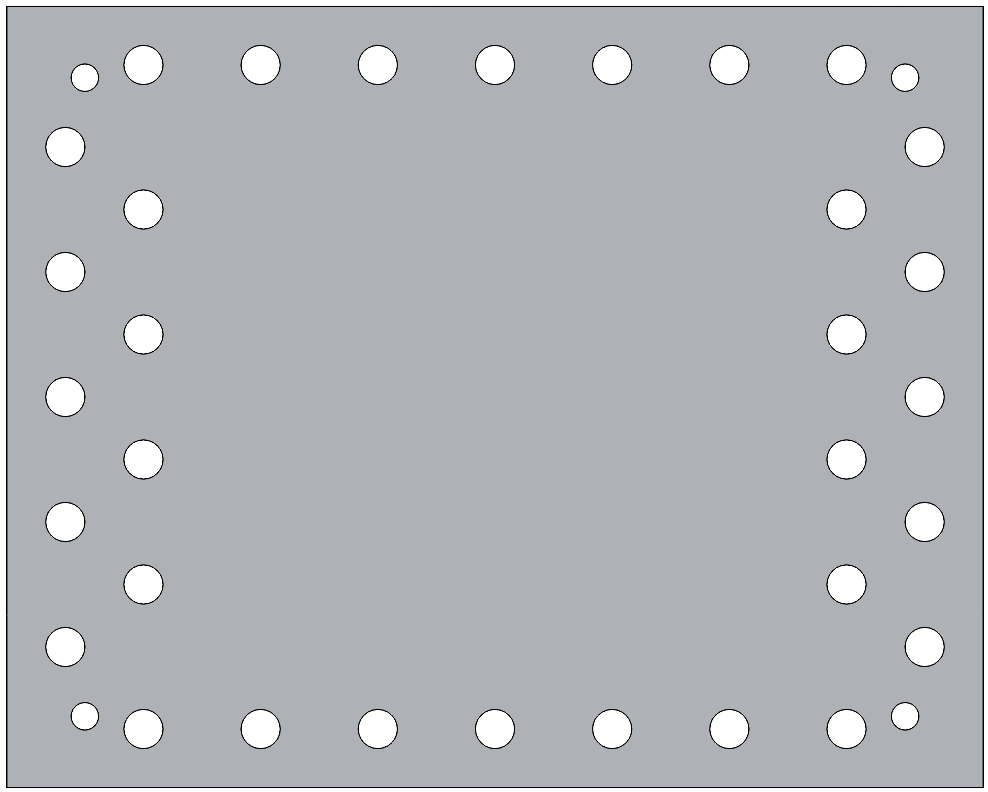
\includegraphics[width=.8\linewidth]{Sections/6 Detaljeløsning/Media/bundplade.png}
         \caption{Illustration af bundplade set oppe fra.}
       \label{fig: bundplade}
    \end{subfigure}
    \begin{subfigure}[b]{0.49\textwidth}
      \centering
      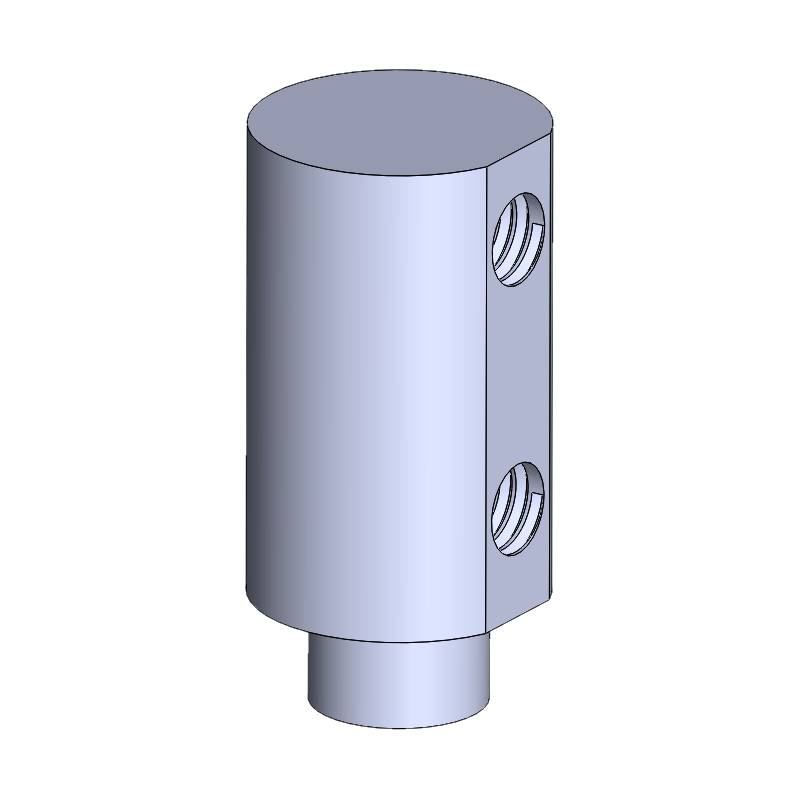
\includegraphics[width=.7\linewidth]{Sections/6 Detaljeløsning/Media/Billeder til indspænding/Gevindholder.png}
      \caption{Gevindholder.}
      \label{fig: gevindholder}
    \end{subfigure}
    \caption{Dele til indspædning}
\end{figure} \plainbreak{-.5}

Indspændingselementer er delene der indspænder emnet. De består af tre dele: en gevindholder (figur \ref{fig: gevindholder}), en \SI{100}{mm} M6 bolt med en gevindhældning på \SI{1}{mm} \parencite{RSComponents2025M6RS} og en PVC endeprop \parencite{Profillageret2025RundProfillageret.dk}. Gevindholderne placeres i et af pladens \SI{10}{mm} huller. De \SI{100}{mm} lange M6 bolte køre igennem gevindholderne, som gør at boltene gradvist spændes mod emnet. For at undgå at emnet beskadiges under indspændingen, er der monteret endeprop på boltenes ende der har kontakt med emnet.

% Skrive om hvor vi har valgt et frirum 3mm. Det med at bolten skal kunne dreje uden problemer.
% To huller for frihed
% Valg for at gøre den rund. Kom ind på optimale fremstilling, samt man kan dreje den så den passer til emener der har skæve former.


For at tage højde for forskellige emne højder, er gevindholderen udforment med to gevind huller, hvilket betyder der kan vælges mellem de to huller alt efter emne højde. Det nederste hul har en fri højde fra pladen på \SI{3}{mm}, for at sikre at bolten ikke kommer i kontakt med pladen, under indspænding. Derudover er frihøjden også valgt ud fra bolten ikke skal være besværlig for forbrugen at tilgå.
Gevindholderens runde form er valgt på baggrund af henholdvis fremstillingsårsager, samt en evne til at kunne passe til emner med skræve former. Ved emner hvor dets sider ikke ligger parallelt med pladens sider, muliggøre gevind holderens cylindriske form, at den kan vinkles til at give den mest optimale kontaktflade med emnet.


Til produktet medfølger seks indspændings elementer, hvortil to af dem er tiltænkt som reserve, eller til tilfælde med ikke prismatiske emner. Det er derved tiltænkt at emner indspændes med to indspændingselementer, som vist på figur \ref{fig: indspænding}. 

\begin{figure}[H]
    \centering
    \begin{subfigure}[b]{0.48\textwidth}
    \centering
         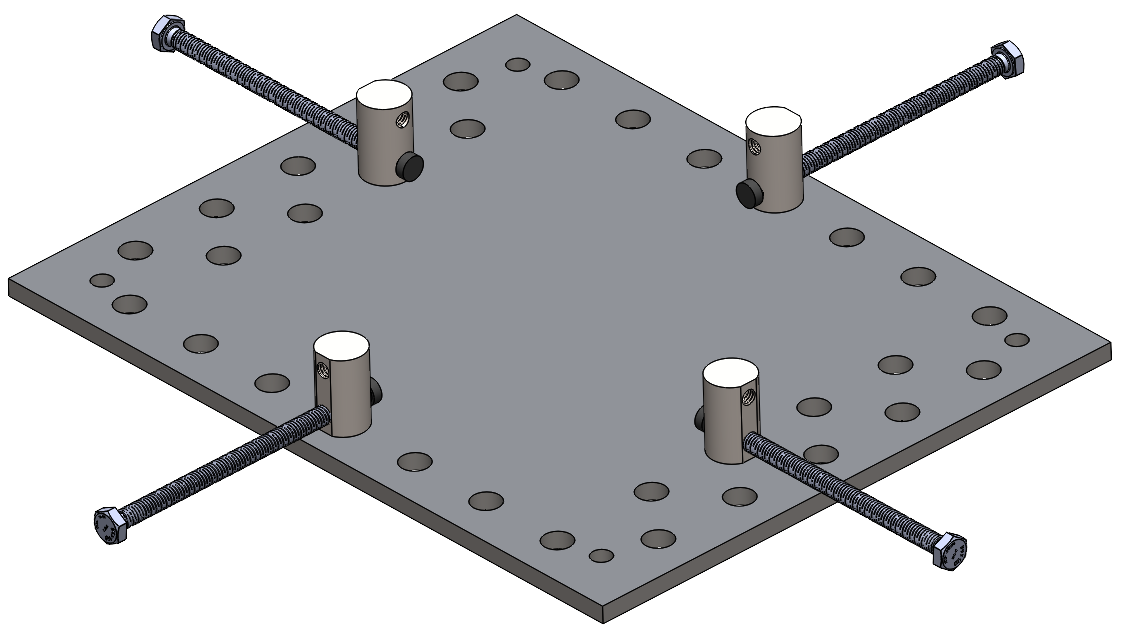
\includegraphics[width=0.9\linewidth]{Sections/6 Detaljeløsning/Media/Indspænding lav.png}
     \caption{Laveste position}
      \label{fig: indspænding lav}
    \end{subfigure} 
    \begin{subfigure}[b]{0.48\textwidth}
    \centering
        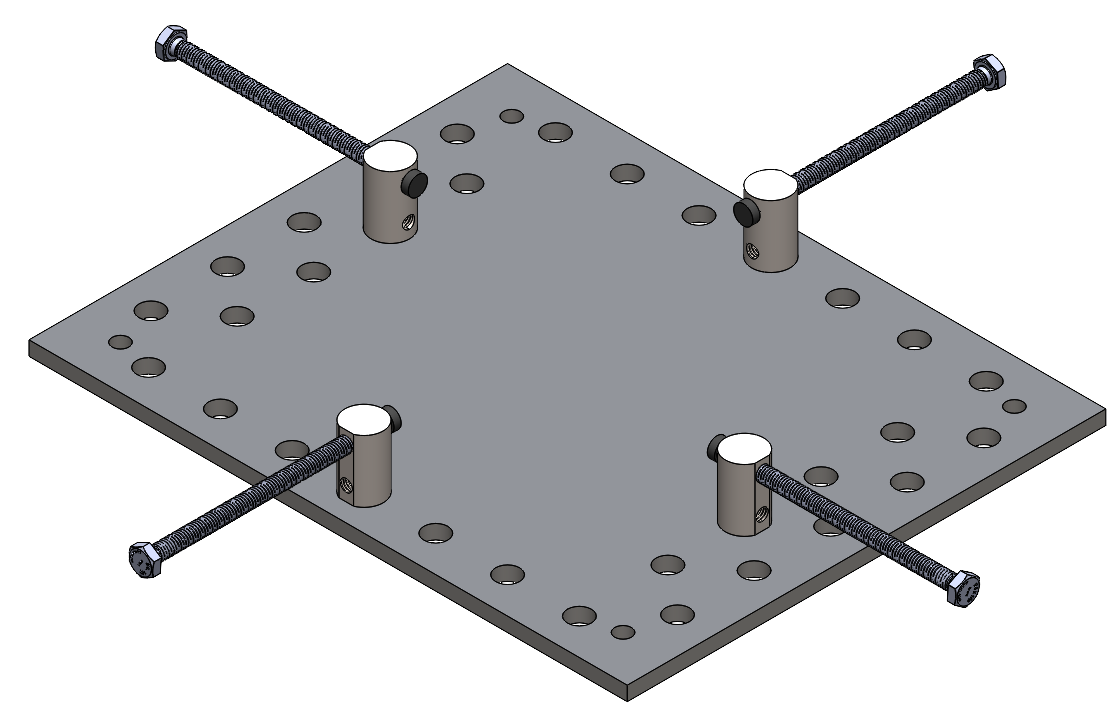
\includegraphics[width=0.9\linewidth]{Sections/6 Detaljeløsning/Media/Indspænding høj.png}
     \caption{Højeste position}
      \label{fig: indspænding høj}
    \end{subfigure}
    \caption{Opstilling af indspændingen hvor bolten er i henholdsvis den laveste og højeste position. Arbejdstegninger kan ses i bilag \ref{Bilag - arbejdstegniner}}
    \label{fig: indspænding}
\end{figure} \plainbreak{-.5}

Bundpladen er $\SI{270}{mm} \times \SI{220}{mm} \times \SI{6}{mm}$, og har en volumen på  $ 340,4 \cdot 10^{-9} \SI{}{m^3}$ der med en densitet på $\approx \SI{7900}{kg \cdot m^{-3}}$ giver en vægt på $\approx \SI{2,8}{kg}$. 

\plainbreak{2}
\section{Fremstilling og prissætning} \label{Fremstillingsmetoder}
Til fremstillingen af produktet kræves der en række forskellige fremstillingsmetoder. I følgende afsnit udvælges enkelte dele hvorefter der beskrives hvilke fremstillingsprocesser disse dele skal igennem før de kan monteres på det endelige produkt. Produktet gør brug af dele lavet ved en række metoder, bland andet ekstrudering, som beskrives i \ref{alu Ekstrudering} herunder, samt dele lavet ved spåndtagning.


\subsection{Fremstilling af monteringsblok} % Ved ikke helt hvad jeg skal kalde dette kapitel
De dele der skal laves internt kan laves ved brug af CNC fræsere og drejebænke. Disse dele vil alle blive lavet af EN-AW 6082 - T6, denne aluminiumslegering har god styrke, bearbejdelighed og pris. Nogle af delene vil være lettere at lave ved hjælp af et "rotary table", dette er en monteringsblok man sætter på fræserens bord, der tillader at rotere emnet. Dette bruges for at mindske hvor gange emnet skal afmonteres for at bearbejde det. Hver gang emnet fjernes fra indspændingen skal maskinens koordinatsystem nulstilles, hvilket gør det sværere at opnå præcision. Herunder gennemgås en mulig måde hvorpå monterings blokken kan fremstilles, det er vigtigt at pointere at dette ikke nødvendigvis er den bedste måde at fremstille delen på, da der mangler viden i projektet om fremstilling. 

\begin{figure}[H]
    \begin{subfigure}[b]{0.48\textwidth}
        \centering
        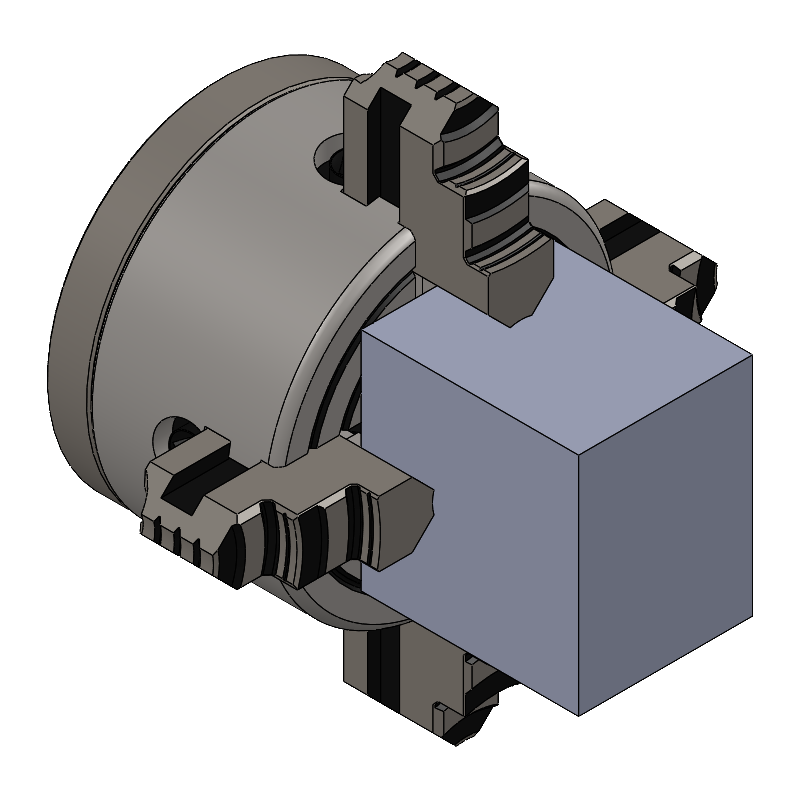
\includegraphics[width=0.8\linewidth]{Sections/6 Detaljeløsning/Media/StepByStep/Step 0.png}
        \caption{Tilskårede materiale fastspændt i chuncken, der er monteret i et rotary table.}
        \label{fig:Step0}
    \end{subfigure}
    \hfill
    \begin{subfigure}[b]{0.48\textwidth}
        \centering
        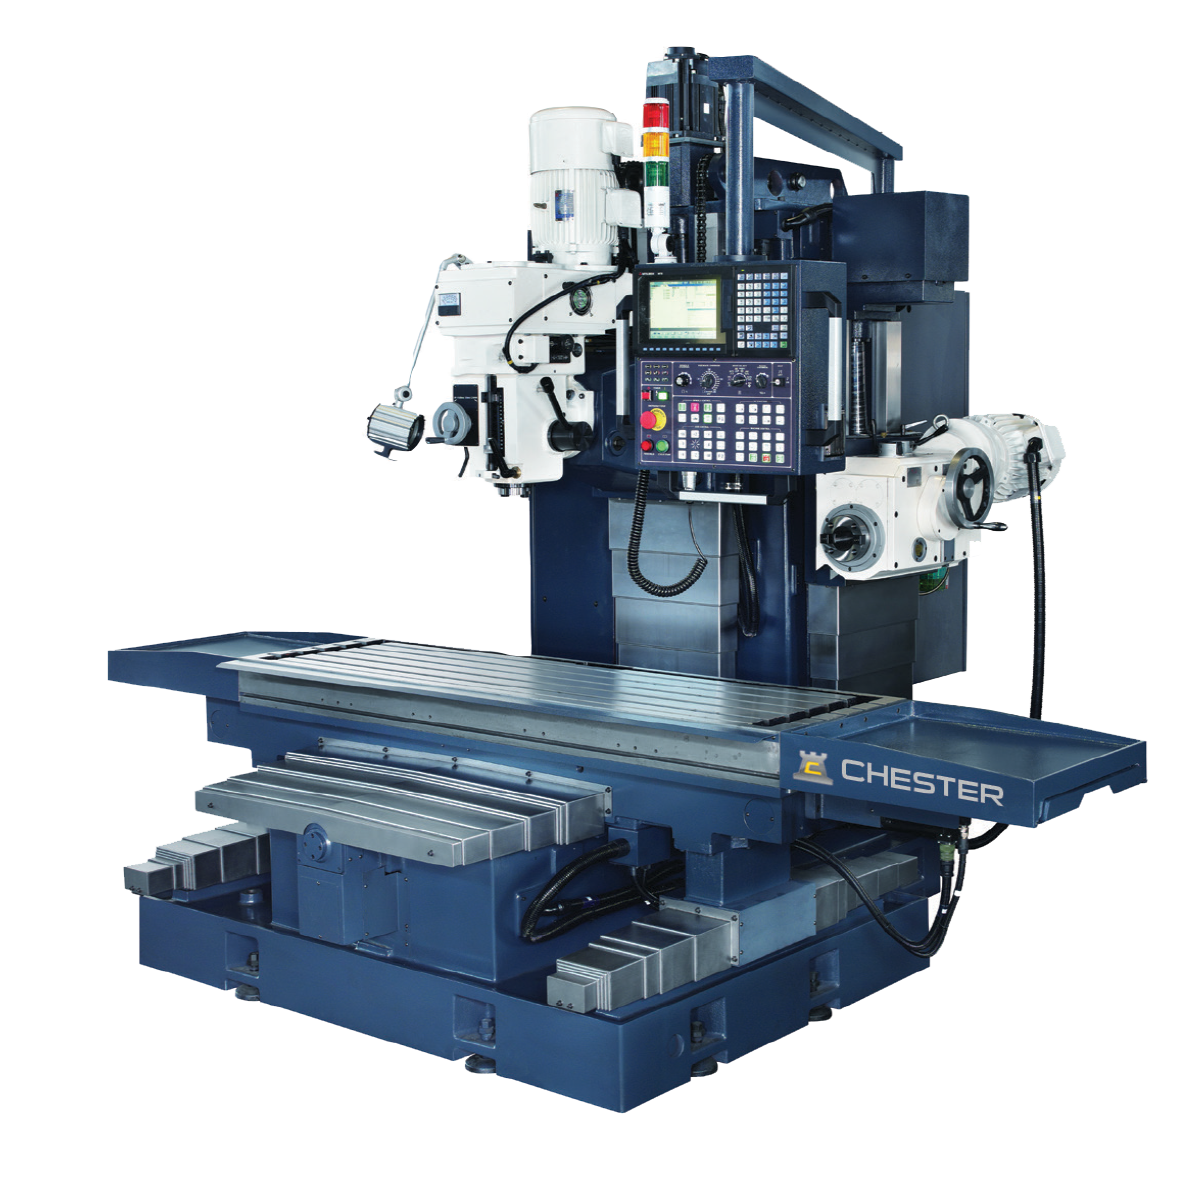
\includegraphics[width=0.8\linewidth]{Sections/6 Detaljeløsning/Media/Vertical-Horizontal-Bed-Type-CNC-Milling-Machine-•-Chester-•-GM1500VS-3222663431.png}
        \caption{Eksempel på en vertikal fræser fra \parencite{CHESTER2025GM1500VSTools}}
        \label{fig:VerticalMill}
    \end{subfigure}
    \\
    \begin{subfigure}[b]{0.48\textwidth}
        \centering
        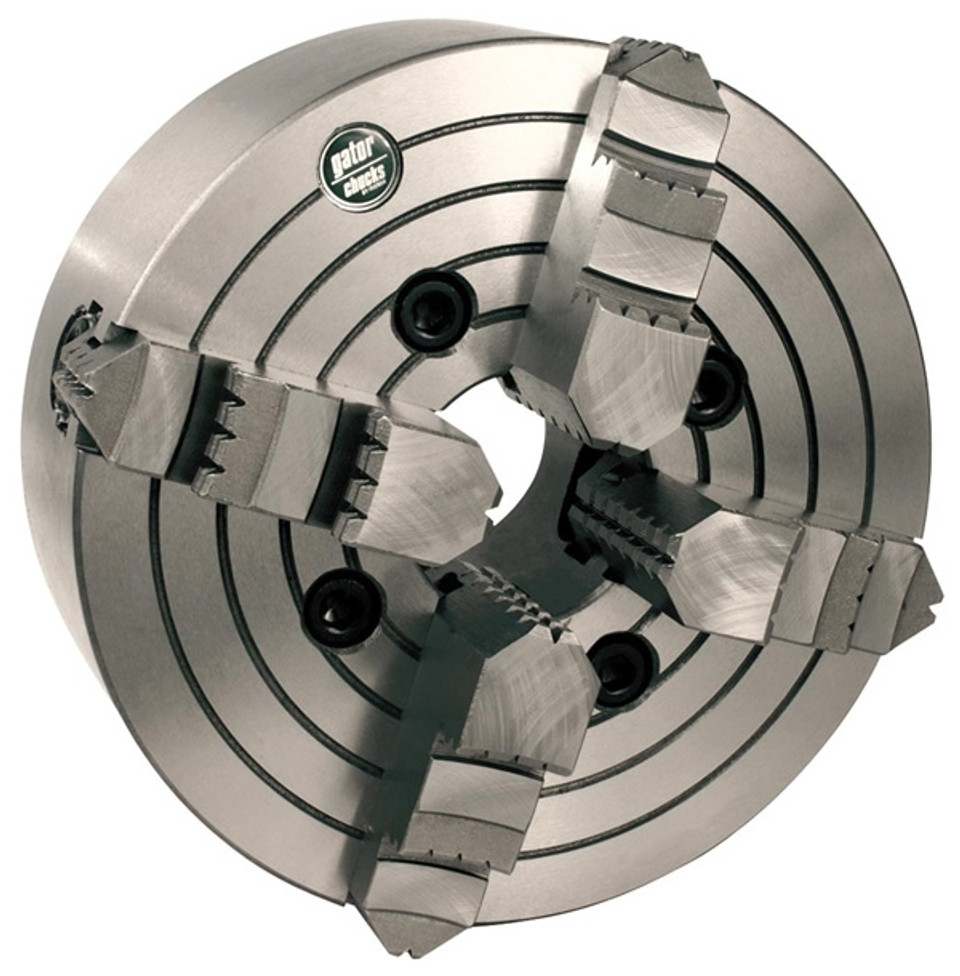
\includegraphics[width=0.8\linewidth]{Sections/6 Detaljeløsning/Media/63-718-004-gator__55302.1565719491-1329413139.jpg}
        \caption{Eksempel på en 4 Jaw chuck fra Gator \parencite{PennToolCo.2025GatorInc}}
        \label{fig:Chuck}
    \end{subfigure}
    \hfill
    \begin{subfigure}[b]{0.48\textwidth}
        \centering
        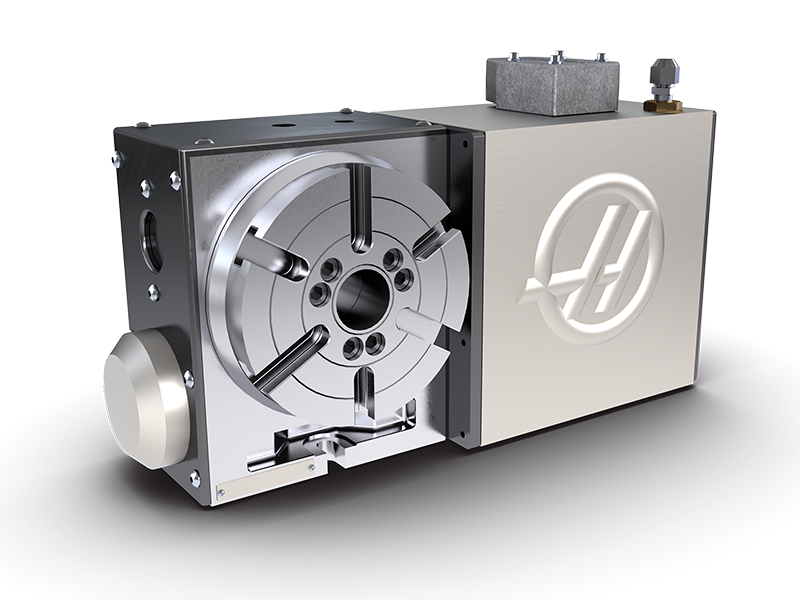
\includegraphics[width=0.9\linewidth]{Sections/6 Detaljeløsning/Media/rotarytable.png}
        \caption{Eksempel på Rotary Table fra \parencite{Haas2025RotaryTables}}
        \label{fig:RotTable}
    \end{subfigure}
\caption{Herunder ses eksempler på det nødvendige maskineri samt udgangspunkter for processen.}
\end{figure} \plainbreak{-.5}

Delen starter som en \(\SI{55}{mm}\) \(\times\) \(\SI{55}{mm}\) \(\times\) \(\SI{55}{mm}\) blok af aluminium 6082-T6 der skæres ud og planes. Man står nu med en blok der er klart til at blive behandlet. Den indspændes i en 4-jaw chuck ((\ref{fig:Chuck}) der er sat i et rotary table (\ref{fig:RotTable})). Herunder ses processen trinvis. For mange af disse trin fjernes størstedelen af materialet ved at tage grove og mindre præcise cuts, efterfulgt af finere og mere præcise cuts, der fjerner mindre materiale.



\begin{figure}[H]
    \centering
    % First row of images
  %  \begin{minipage}[t]{\textwidth}
        \begin{subfigure}[t]{0.32\textwidth}
            \centering
            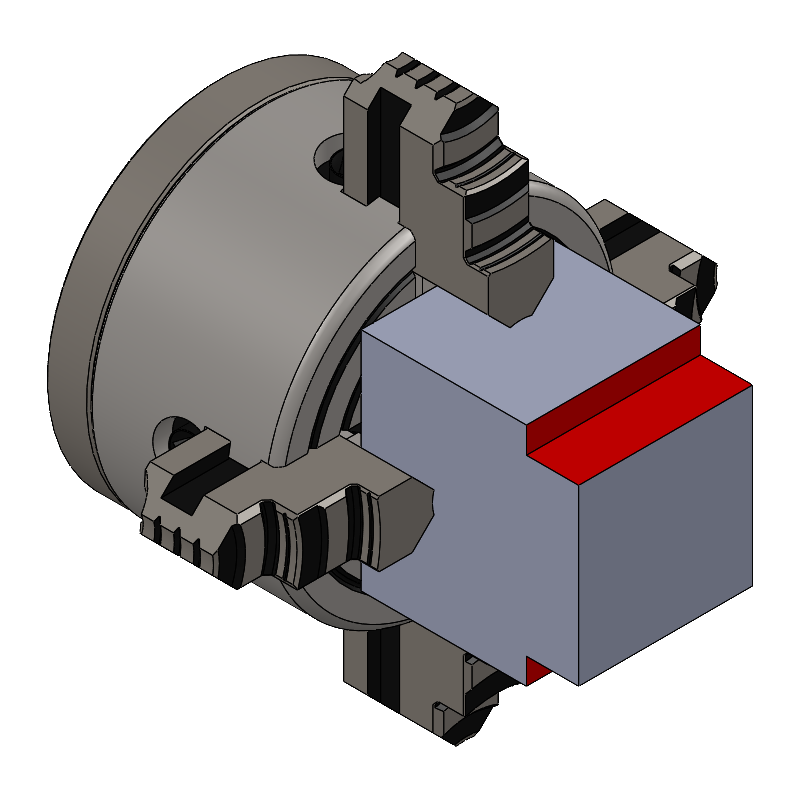
\includegraphics[width=0.9\linewidth]{Sections/6 Detaljeløsning/Media/StepByStep/Step 1.png}
            \caption{Et $\SI{6}{\milli\meter}$ dybt og $\SI{12}{\milli\meter}$ bredt område fræses væk med endefræsning; dette gøres på begge sider.}
            \label{fig:Step1}
        \end{subfigure}
        \hfill
        \begin{subfigure}[t]{0.32\textwidth}
            \centering
            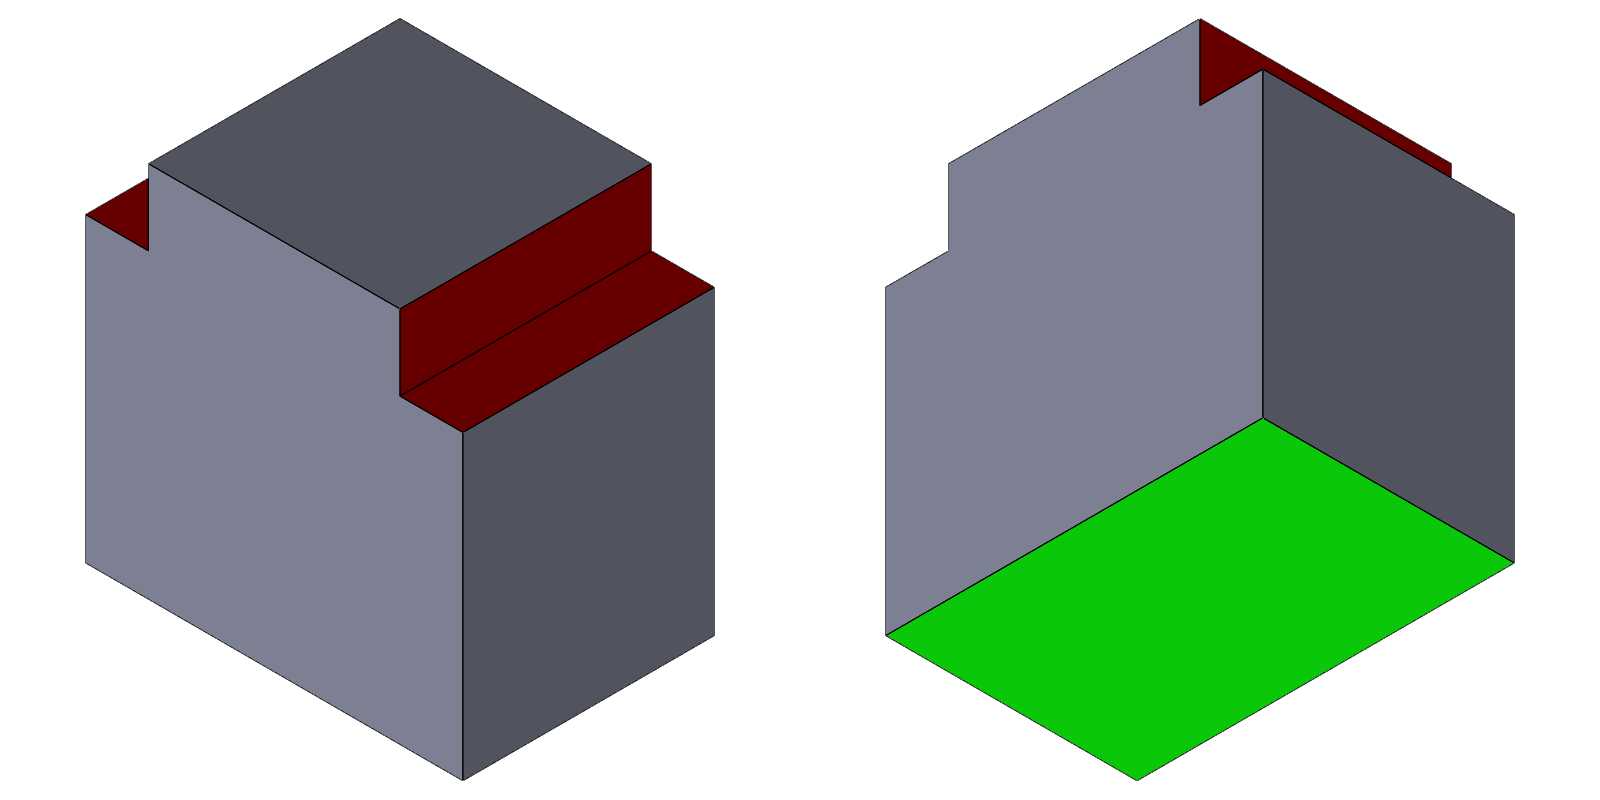
\includegraphics[width=0.9\linewidth]{Sections/6 Detaljeløsning/Media/StepByStep/Step 2.png}
            \caption{Med et fasværktøj fræses en $\SI{6}{\mm} \times \SI{45}{\degree}$ fas som vist ovenfor, dette udføres på begge sider.}
            \label{fig:Step2}
        \end{subfigure}
        \hfill
        \begin{subfigure}[t]{0.33\textwidth}
            \centering
            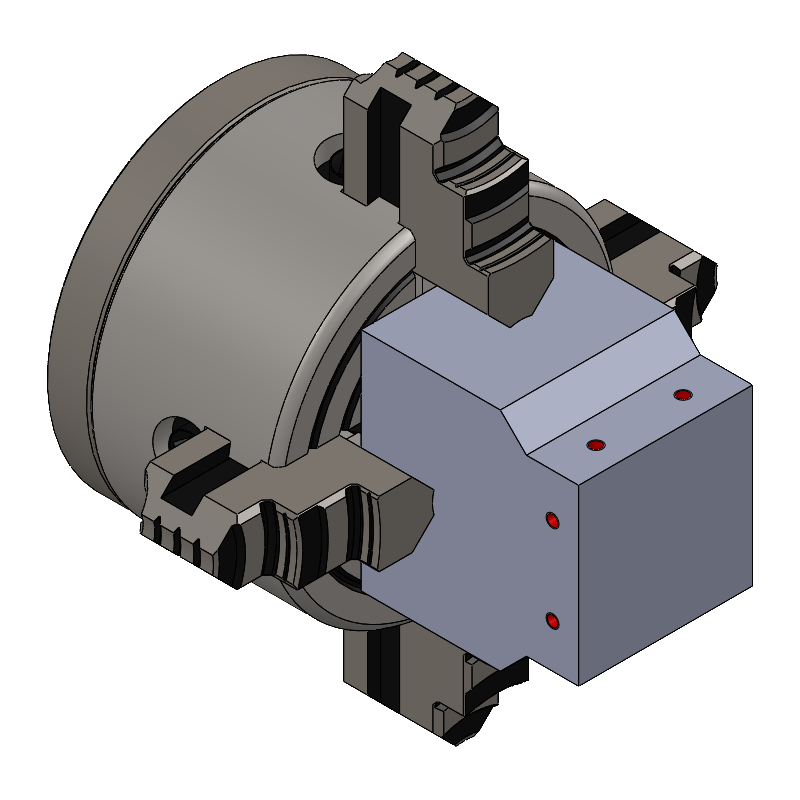
\includegraphics[width=0.9\linewidth]{Sections/6 Detaljeløsning/Media/StepByStep/Step 3.png}
            \caption{Gevindhuller fremstilles ved først at bore et hul, i dette tilfælde med et $\SI{2.5}{\milli\meter}$ bor, hvorefter der anvendes en gevindtap. Denne proces gentages på alle fire sider.}
            \label{fig:Step3}
        \end{subfigure}
   % \end{minipage}
    
    \vspace{1em}
    %\begin{center}
      %  \small Emnet fjernes og vendes for at blive fastspændt ved den netop bearbejdede flade
   % \end{center}
  %  \vspace{1em}
    
    % Second row of images
  %  \begin{minipage}[t]{\textwidth}
        \begin{subfigure}[t]{0.32\textwidth}
            \centering
            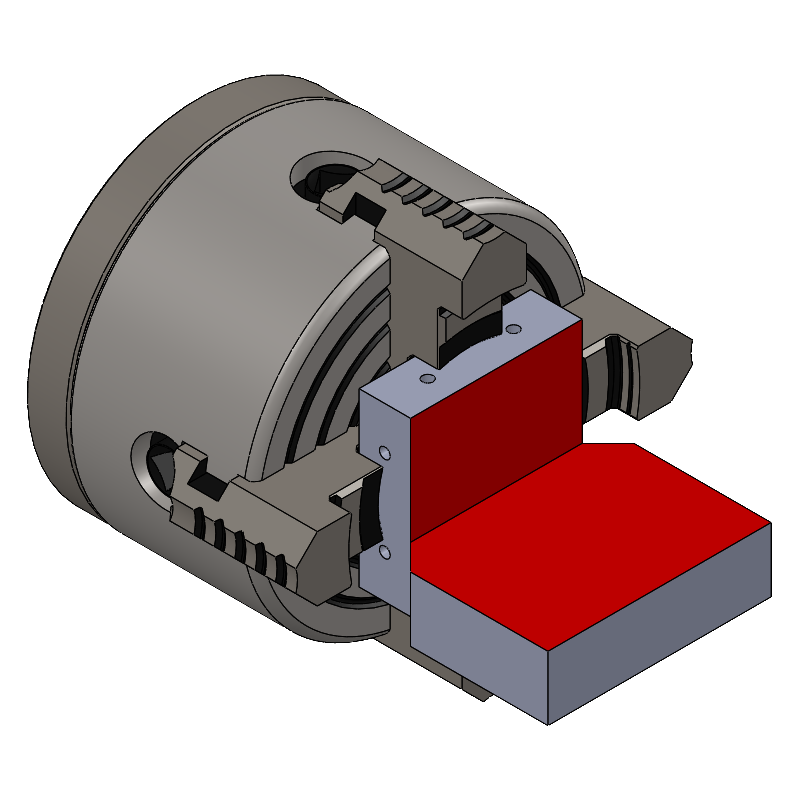
\includegraphics[width=0.9\linewidth]{Sections/6 Detaljeløsning/Media/StepByStep/Step 4.png}
            \caption{Dette er et omfattende trin, som kræver mange snit med en endefræser. Dette kræver opmærksomhed for at undgå at deformere emnet, da en stor mængde materiale skal fjernes}
            \label{fig:Step4}
        \end{subfigure}
        \hfill
        \begin{subfigure}[t]{0.32\textwidth}
            \centering
            \includegraphics[width=0.9\linewidth]{Sections/6 Detaljeløsning/Media/StepByStep/Step 5.png}
            \caption{Emnet roteres, og igen anvendes et fasværktøj, dimensionerne er de samme som i trin 2.}
            \label{fig:Step5}
        \end{subfigure}
        \hfill
        \begin{subfigure}[t]{0.32\textwidth}
            \centering
            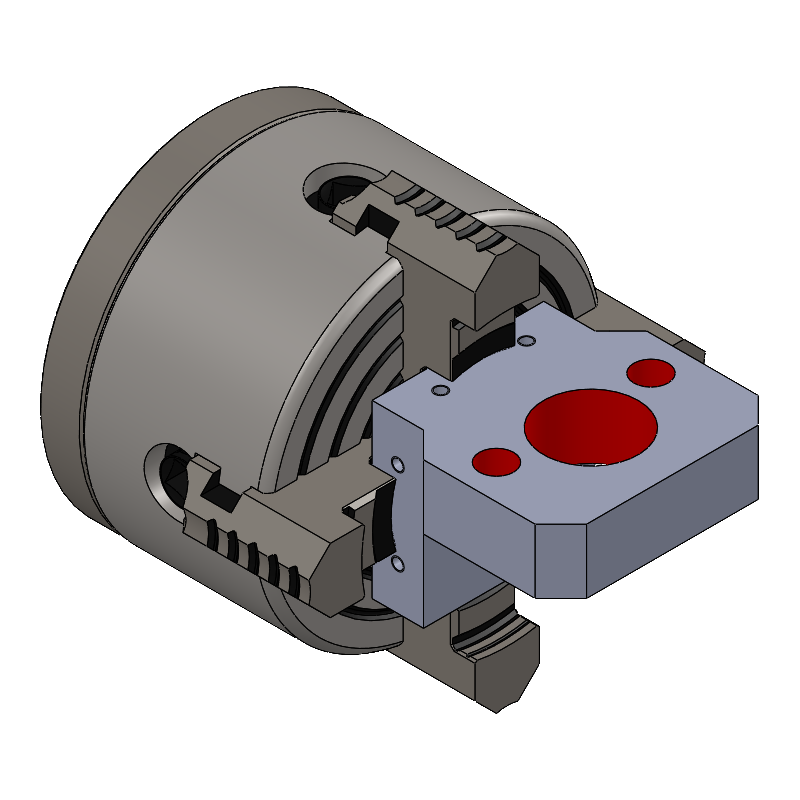
\includegraphics[width=0.9\linewidth]{Sections/6 Detaljeløsning/Media/StepByStep/Step 6.png}
            \caption{Det centrale hul kan bores i ét trin hvis et \SI{22}{mm} bor ejes, ellers må det fræses ud. De to mindre huller kræver en plan bund, så værktøjs udvalget bestemmer processen. Selvom fladbundsbor findes, kan hullerne også fræses.}
            \label{fig:Step6}
        \end{subfigure}
   % \end{minipage}
    
    \vspace{1em}
    
    % Third row of images
    %\begin{minipage}[t]{\textwidth}
        \begin{subfigure}[t]{0.32\textwidth}
            \centering
            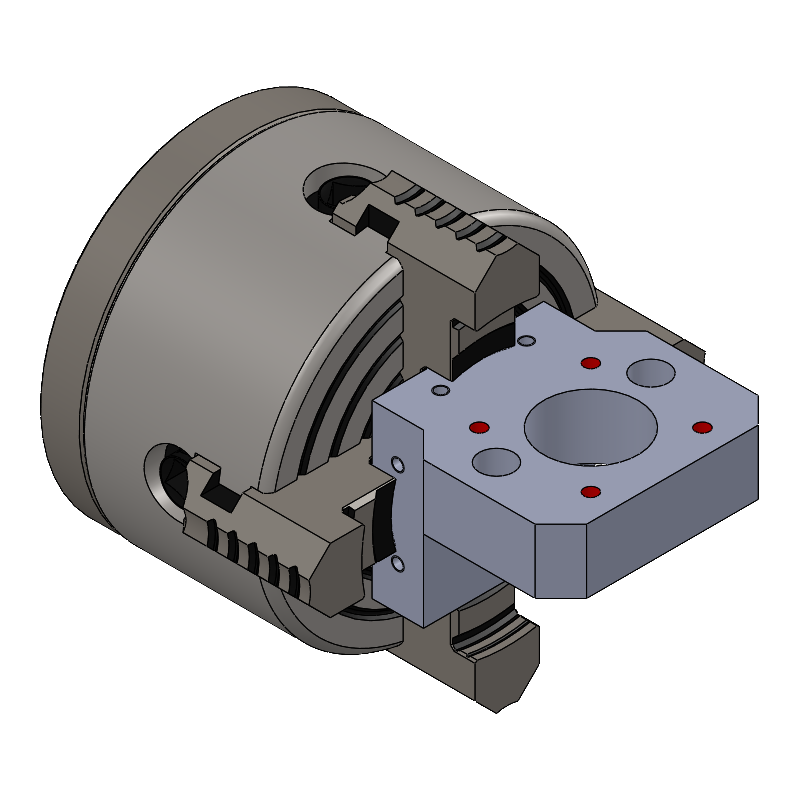
\includegraphics[width=0.9\linewidth]{Sections/6 Detaljeløsning/Media/StepByStep/Step 7.png}
            \caption{I modsætning til de tidligere huller er disse ikke med gevind, men de er forsænkede. Først bores et frigangshul til M3 med en diameter på $\SI{3.4}{\milli\meter}$. Da det er gennemgående huller kan de bare bores.}
            \label{fig:Step7}
        \end{subfigure}
        \hfill
        \begin{subfigure}[t]{0.32\textwidth}
            \centering
            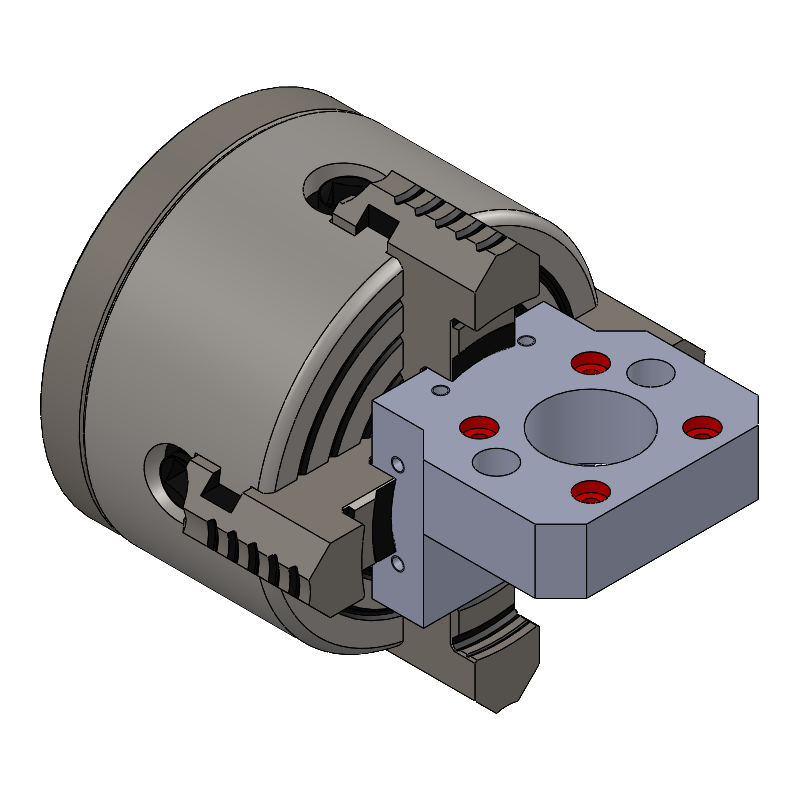
\includegraphics[width=0.9\linewidth]{Sections/6 Detaljeløsning/Media/StepByStep/Step 8.png}
            \caption{Næste trin er forsænkningerne. For de anvendte bolte er en forsænkning på $\SI{6.40}{\milli\meter}$ i diameter og $\SI{2.4}{\milli\meter}$ i dybde nødvendig. Dette kan udføres med en forsænker, som centreres i de tidligere borede huller.}
            \label{fig:Step8}
        \end{subfigure}
        \hfill
        \begin{subfigure}[t]{0.32\textwidth}
            \centering
            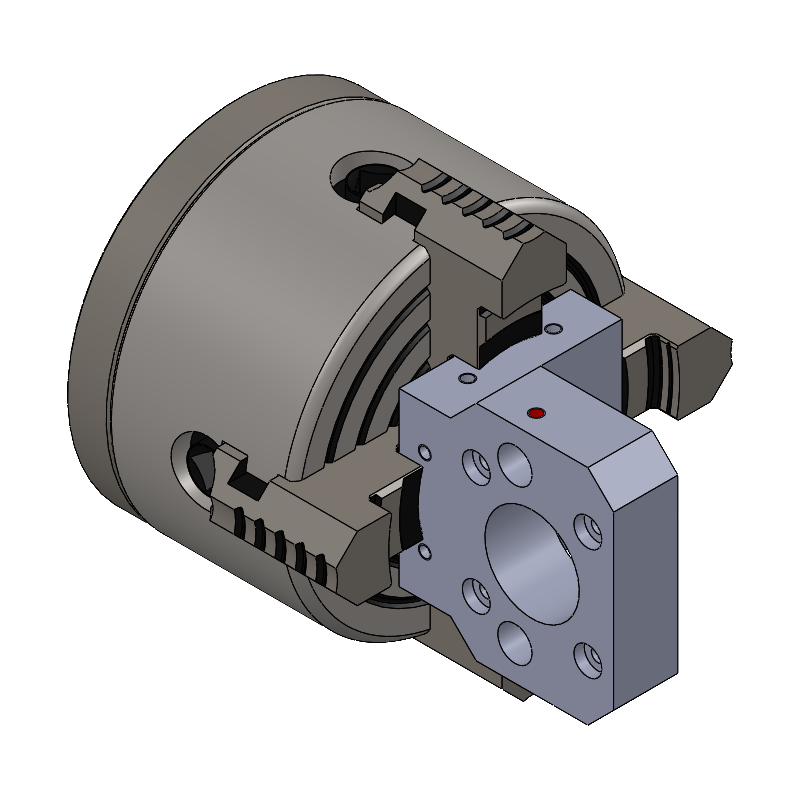
\includegraphics[width=0.9\linewidth]{Sections/6 Detaljeløsning/Media/StepByStep/Step 9.png}
            \caption{Det sidste trin er hul og gevind til M4-pinol skruerne der fastgør akslerne. Processen er den samme som i trin 3, blot med en M4-gevindtap og et $\SI{3.25}{\milli\meter}$ bor.}
            \label{fig:Step9}
        \end{subfigure}
   % \end{minipage}
    
    \caption{Trin-for-trin fremstillingsproces af emnet. Emnet fjernes og vendes mellem \textit{(c)} og \textit{(d)}, for at blive fastspændt ved den netop bearbejdede flade}
    \label{fig:stepbystep}
\end{figure}


%Gevindholderen til indspændingssystemet (se figur \ref{fig:Gevindholder-frem}) er fremstillet af en rustfri stålstang og udgør det faste element, som M6-boltene skrues ind i, når emnet skal fastholdes på bundpladen. Gevindholderen er dreget i ét stykke rustfrit stål, så dens ydre cylindriske form med diameter på 16 mm let kan vinkles mod emnet og fordele spændekraften jævnt, også på skrå overflader. 
%Under fremstilling skæres en Ø16 stang til, hvorefter den på en CNC-drejebænk bearbejdes med en indsnævring på 10 mm i den ene ende, så den passer i de tilsvarende huller på arbejdspladen. I en CNC-fræser  bearbejdes den med to gennemgående M6-gevind, med en frihøjde på henholdsvis 3 og 16 mm indsnævringen og derved arbejdspladen. Efter gevindskæring slibes og affases enderne for at fjerne grader, og hele holderen poleres for at beskytte gevindets tolerance ($\pm$ 0,1 mm) og sikre problemfri boltføring. 



%\begin{figure}[H]
%    \centering
%    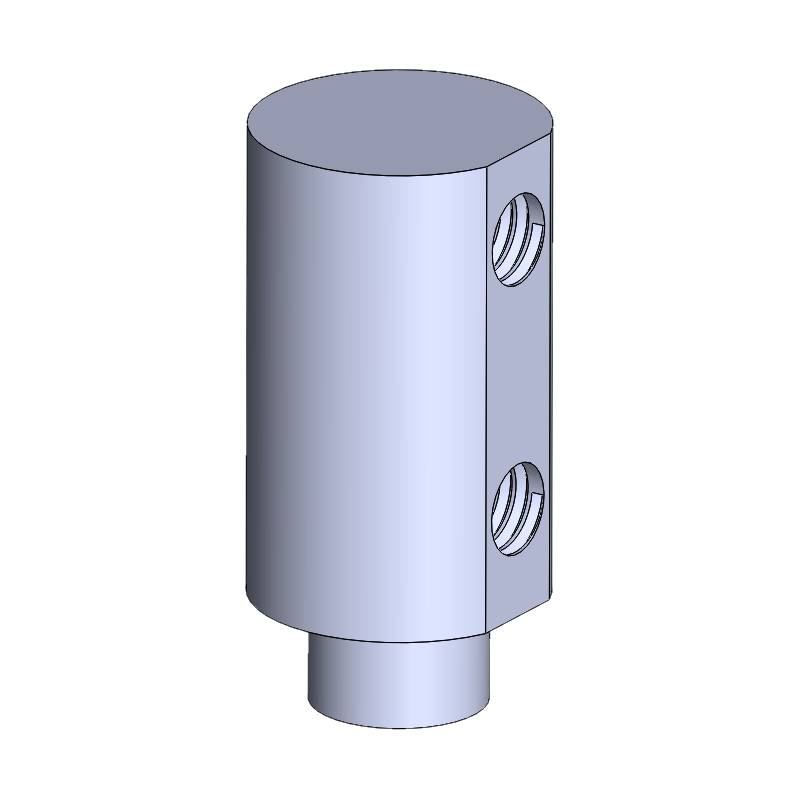
\includegraphics[width=0.5\linewidth]{Sections/6 Detaljeløsning/Media/Billeder til indspænding/Gevindholder.png}
%    \caption{Gevindholder}
%    \label{fig:Gevindholder-frem}
%\end{figure}

\subsection{Aluminiums profiler} \label{alu Ekstrudering} \plainbreak{-.5}
Til konstruktion af robottens stativ er der anvendt T-slotprofiler i aluminium (se figur \ref{fig:T-slot profil}), som er fremstillet ved ekstrudering. Ekstrudering er en kontinuerlig produktionsproces, hvor et opvarmet aluminiumsemne kaldet en billet - presses gennem en form (matrice) der er profilens ønskede tværsnit. Ved hjælp af højt tryk og temparatur opnås en ensartet, langstrakt profil med præcis geometri.\parencite{Johnson1962TheExtrusion} 

Processen begynder med forvarmning af aluminiumsbilletten til cirka 450-500 grader °C, hvorefter den presses gennem matricen med en hydraulisk presse. Når profilen forlader matricen, afkøles den kontrolleret med luft eller vand for at opretholde den dimensionelle stabilitet. Efter afkøling rettes profilen mekanisk, og overskydende materiale i enderne fjernes. Til sidst varmebehandles profilerne (typisk T5 eller T6-hærdning) for at opnå den ønskede styrke og hårdhed. Til applikationen i projektet tages disse lange profiler og tilskæres de ønskede længder der skal bruges. \parencite{Johnson1962TheExtrusion} 
 
\begin{figure}[H]
    \centering
    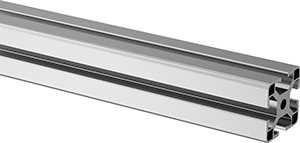
\includegraphics[width=0.35\linewidth]{Sections/6 Detaljeløsning/Media/T-slots.png}
    \caption{T-slot alu profilrør. \parencite{McMaster-Carr2025T-SlottedRails}}
    \label{fig:T-slot profil}
\end{figure} \plainbreak{-.5}


\plainbreak{0.2}
\subsection{Samling} \label{samling}
Ekstrudering er en økonomisk og præcis fremstillingsmetode, der muliggør høj gentagelsesnøjagtighed og lav materialespild \parencite{Johnson1962TheExtrusion}. Desuden er aluminium velegnet til robotstativet grundet dets lave vægt og tilstrækkelige mekaniske styrke, se afsnit. 

Ses der på den samlede konstruktion af robotten er den primære samlingsmetode bolte. Hele robotstrukturen er opbygget som en modulær skruesamling, hvor alle mekaniske komponenter, fra T-slot-rammen over følgestænger og motorbeslag til doseringshoved, fastgøres med standard skruer. På aluminiumsprofilerne anvendes T-slot-notsten, som glider ind i profilens riller, hvorefter en skrue bruges til at montere beslag, motorer og så videre. Hvordan dette samles kan ses i bilag \ref{Bilag - arbejdstegniner}.

\begin{table}[H]
\setlength{\tabcolsep}{20pt}
 \centering
  \caption{Værktøjsliste}
 \begin{tabular}{|l l|} \hline
  \multicolumn{2}{|c|}{\cellcolor{aaublue} \color{white} \textbf{Værktøjsliste}}  \\\hline
 \rowcolor{gray!10} \multicolumn{1}{|c}{\textbf{Navn}} &  \multicolumn{1}{c|}{\textbf{Anvendelsessted}}  \\\hline

  10 mm fastnøgle & Indspænding  \\\hline
  4 mm umbracho nøgle & \makecell{Indspænding \\ Samling af stellet \\ Lineær bevægelse}  \\\hline
  2 mm umbracho nøgle & \makecell{Lineær bevægelse }  \\\hline
 
 \end{tabular}
 \label{tab: værktøjsliste}
\end{table}

Til samling af speckle pattern robotten benyttes tre standard værktøj, som fremgår af tabel \ref{tab: værktøjsliste}.






\plainbreak{2}
\subsection{Prissættelse} \label{Stykliste}
Styklisten udgør en samlet oversigt over alle de komponenter og materialer, der indgår i den mekaniske konstruktion af løsningen. Den er udarbejdet med henblik på at give et overblik over nødvendige dele til samling af produktet. Hver komponent er opført med tilhørende betegnelse, antal og  materiale samt pris. Da produktet fokusere på de mekaniske aspekter, er styklisten afgrænset til de dele, der er direkte relateret til konstruktionen og den mekaniske funktionalitet af robotten. Elektriske komponenter of softwaredele er ikke inkluderet, da disse ligger ude for projektets afgrænsning (se afsnit \ref{Afgrænsning}). Styklisten danner grundlag for både kostestimering og fremstillingsforberedelse af en eventuel prototype. Den samlede stykliste kan ses i bilag \ref{Bilag - stykliste}. Yderligere er enkelte dele blevet estimeret i pris og arbejdstimer af MEB Smedie og Maskinværksted ApS, de korresponderende mails hertil kan ses i bilag \ref{Mail - prisestimat}. Baseret på dette er overslaget på prisen 88.886 DKK.






\plainbreak{2}
\section{Vurdering af præstationskrav} \label{vurdering af krav}
Efter udarbejdelsen af kravspecifikation og udviklingen af det endelige koncept er det essentielt at vurdere, i hvilken grad designet lever op til de opstillede præstationskrav. Denne vurdering har til formål at klarlægge, hvorvidt den mekaniske løsning er egnet til at opfylde de krav, der blev fastlagt ud fra de behov der blev fundet i problemanalysen (se afsnit \ref{Endelige kravspecifikationer}). Graden hvor i kravene er opfyldt, vil blive vist i tabel \ref{tab: vurdering af krav} herunder. Følgende tabel klargøre hvor vidt der leves op til de forskellige krav, samt angiver i hvilede afsnit der er blevet arbejdet med hvert krav. 

\renewcommand{\arraystretch}{1.4}
\begin{table}[H]
    \centering
    \small
     \caption{Præstationskrav. Relativ vigtighed ($\Omega$). \textbf{++} betyder at præstationskravet er opfyldt med sikkerhed. \textbf{+} betyder at præstationskravet er vurderet opfyldt med små usikkerheder. \textbf{/} betyder at der er for stor usikkerhed, til at bestemme om præstationskravet er opfyldt. \textbf{-} betyder at præstationskravet ikke er opfyldt. Afsnit kolonnen angiver hvor i rapporten der er blevet taget højde for kravet. }
      \begin{tabular}{|p{11cm}|c|c|c|} \hline
     \multicolumn{1}{|c}{\cellcolor{aaublue} \textcolor{white}{\textbf{Præstationskrav}}}  &  \multicolumn{1}{|c|}{\cellcolor{aaublue} \textcolor{white}{Afsnit}} &  \multicolumn{1}{|c|}{\cellcolor{aaublue} \textcolor{white}{Vurdering}} \\ \specialrule{0pt} {0.5pt}{0pt} \hline
        1. Justerbar prikstørrelse fra \SI{0,1}{mm}-\SI{1,0}{mm}  & \ref{Prikplacering} & {$+$}\\ \hline
        2. Variation i størrelse af påsat prik på maksimum $\SI{\pm0,05}{mm}$ &  \ref{Prikplacering} & {$+$}\\ \hline
        3. Acceptabel afvigelse af planlagt prikplacering på $\SI{\pm0,1}{mm}$ &   \ref{Præcisions beregninger} & {$+$}\\ \hline
        4. Størrelse af arbejdsområde $\SI{200}{mm} \times \SI{150}{mm}  \times\SI{50}{mm} $  & \ref{Indspænding} & {$++$}\\ \hline
        5. Maks flytning af emne under påføring af speckle pattern på \SI{0,01}{mm}  &  \ref{Indspænding} & {$+$}\\ \hline
        6. Mængde af forskellige påføringsmidler til koncept på minimum 2  & \ref{Prikplacering} & {$++$}\\ \hline
        7. Minimum greyscaleværdi på 100 point &  \ref{Prikplacering} & {$/$} \\ \hline
        8. Maksimalt tidsforbrug på prikplacering pr. cm$^2$ på 30 sekunder  &  \ref{Kinematisk analyse} & {$+$}\\ \hline
        9.  Maks brugerinteraktion under påføring af speckle pattern på 1 min & - & {$+$}\\ \hline
        10. Maksimal tidsforbrug på opsætning af robot på 10 min & \ref{Indspænding} & {$+$}\\ \hline
        11. Mængde af forskellige værktøjer til samling på 5  stk.  & \ref{Stykliste} & {$++$}\\ \hline
        12. Mængde af specialværktøj til samling af robot på maksimum 1 stk.& \ref{Stykliste} &{$++$}\\ \hline
    \end{tabular}
    \label{tab: vurdering af krav}
\end{table} 


 \plainbreak{1}      
Præstationskrav 1 og 2 vurderes begge til 1 plus. Dette er gjort da værktøjet der laver disse prikker kommer udefra, og de mål der bliver angivet ikke nødvendigvis er lavet på de metalflader og det miljø der skal bruges i DIC sammenhæng (Se afsnit \ref{Prikplacering}).

Præstationskrav 3 har fået ét plus, da der her igen er små usikkerheder i forhold til løsningen. Der er lavet udregninger på udbøjning under bevægelse som overholdet kravet, der er her ikke taget højde for egenfrekvens og vibration af skruen, som kan føre til komplikationer i bevægelsen (Se afsnit \ref{Præcisions beregninger}).

Præstationskrav 4 og 5 beskriver, vurderes til hhv. to plus og et plus. Arbejdsområdet er sikret sin størrelse med plads til indspændinger, dette er sikret og dermed to plusser. Flytning af emnet har ét plus, da der er lavet indspændinger, der i teorien skal holde emnet fast, dette er ikke testet og er derfor ikke sikkert. (Se afsnit \ref{Indspænding})

Præstationskrav 6 og 7 har fået henholdsvis. to plusser og en skråstreg. Præstationskrav 6 er med sikkerhed løst, da prikværktøjet, PeJV, er egnet til en lang række væsker. Præstationskrav 7, omkring grayscale værdi, kan ikke vurderes, da dette afhænger af baggrundsfarve og malingens farve, og dette er ikke undersøgt i rapporten. (Se afsnit \ref{Prikplacering})

Præstationskrav 8 har fået ét plus. Dette er vurderet ud fra udregningerne fra den kinematiske analyse. Her er der ikke taget hensyn til at flytte massen på skruen, og der er derfor usikkerheder i løsningsgraden. (Se afsnit \ref{Kinematisk analyse})

Det er blevet vurderet at produktets opsætning ikke overstiger de 10 minutter, som præstationskrav 10 frem sætter, samt heller ikke overstiger præstationskrav 9's begrænsning på ét minuts brugerinteraktion. Dog er produktet ikke blevet fremstillet og testet, hvilket betyder det ikke kan konkluders med total sikkerhed at præstationskrav 9 og 10 er opfyldt (Se afsnit \ref{Indspænding}).

Med et brug af blot 3 forskellige standard værktøjer, opfyldes både præstationskrav 11 og 12, hvortil de begge er blevet vurderet til to plusser (Se afsnit \ref{Stykliste}).



%- vurdering af speckle pattern robot ift. HoQ ønsker (bilag \ref{Bilag - Vurdering af speckle patttern robot})










\begin{comment}
1. Prikstørrelse\\ 
Prikkernes minimumsstørrelse er sat til 0,1 mm for at sikre synlighed med det blotte øje i makroskala. Dette krav er løst gennem anvendelsen af PeJV-systemet, som tillader meget præcis dosering af væske. Systemet er er i stand til at placere prikker ned til  0,03 mm i diameter, hvilket opfylder det tekniske krav og sikre anvendeligheden til DIC i den ønskede størrelsesorden (se afsnit \ref{Prikplacering}).  

2. Variation på prikstørrelser\\
Det ønskede krav er, at prikstørrelsesvariationen skulle holdes under $\pm$ 0,05 mm for at sikre et ensartet Vpeckle pattern. Løsningen anvender PeJV-systemet til at opnå kontrolleret og gentagelig dosering af prikker. PeJV-systemet sikrer en lav variation, dog er der ikke gennemført målinger til at dokumentere præcisionen af PeJV-systemet. Da den reelle variation derfor ikke kan verificeres, vurderes kravet som delvist opfyldt, (se afsnit \ref{Prikplacering}).  

3. Variation på prikplacering\\
Kravet om placering med høj præcision (maksimalt $\pm$ 0,1 mm afvigelse) er løst ved hjælp af lineær føring og steppermotorer som muliggører præcis og kontrolleret bevægelse af doseringshovedet. Beregninger i afsnit \ref{Kinematisk analyse af lineær bevægelse} og \ref{beregninger: lineær bevægelse præcision} viser, at systemet kan holde sig inden for den ønskede tolerance margin. Dermed er specifikationen opfyldt.  

4. Størrelse af arbejdsområde\\
 Designet skulle kunne dække et ønsket arbejdsområde på 200 mm x 150 mm x 50mm. Dette krav er løst ved at dimensionere robotten specifikt til dette område, (se kapitel \ref{Detaljeløsning}). Kravet vurderes derfor som opfyldt.  

5. Flytning af emnet under proces\\
For at undgå fejl i speckle pattern’et skal emnet forblive fuldstændigt stationært under prikplaceringen. Dette er løst gennem en simpelt mekanisk indspændingssystem som fastholder emnet under hele processen. Indspændingsløsningen er beskrevet i afsnit \ref{Indspænding} og vurderes til at kunne holde bevægelsen under de ønskede $\pm$ 0,1 mm. Derfor betragtes kravet som opfyldt. 

6. Antal forskellige påføringsmidler\\
Systemet skal kunne understøtte flere forskellige typer blæk eller farvestoffer for at sikre fleksibilitet på tværs af materialer og overflader. Dette er løst gennem valget af PeJV, som kan håndtere væsker med varierende viskositet. Dette gør det muligt at benytte forskellige typer påføringsmidler uden ombygning eller justering. Derved vurderes kravet som opfyldt. 

7. Kontrast mellem prik og baggrund\\
For at sikre præcis billedbehandling i DIC kræves en kontrast på minimum 130 gray-level point mellem prikker og baggrund. Dette opnås ved at anvende sort farve på en hvid eller lys baggrund, hvilket giver høj kontrast og gør prikkerne tydelige. Løsningen vurderes som opfyldt, da et farvemiddel kan vælges der passer til det enkelte materiale. 

8. Tidsforbrug på prikplacering\\
Der er stillet et krav, at systemet skal kunne fremstille 1 cm² på 30 sekunder, for at sikre effektivitet og gøre løsningen konkurrencedygtig i forhold til manuelle metoder. I det færdige design tager det 9,46 sekunder at dække 1 cm² med prikker (se afsnit \ref{Kinematisk analyse af lineær bevægelse}). Systemets bevægelse og dosering foregår automatisk og uden brugerinvolvering, hvilket betyder, at det samlede arbejdstempo opretholdes stabilt. Denne tid vurderes at være passende i forhold til kravets formål og systemets anvendelse. Derfor anses specifikationen som opfyldt.

9. Brugerinvolvering under proces\\
Et vigtigt mål var at minimere brugerinvolvering, således at systemet kunne køre autonomt efter opsætning. Dette er løst gennem et kontrolsystem, der efter kalibrering selv udfører hele prikplaceringen. Brugeren skal kun placere emnet, spænde emnet ind og starte processen. Kravet vurderes som opfyldt. 

10. Tid brugt på opsætning\\
Opsætningstiden skal holdes lav for at gøre systemet effektivt i brug. Dette er løst gennem en simpel indspændingsmekanisme, i kombination med et intuitivt kalibreringssystem via kamera og touchskærm (afsnit \ref{Detalje - kontrolsystem}). løsningen vurderes at opfylde kravet.  

11. Antal værktøjer til samling\\
For at sikre nem samling og vedligeholdelse ønskedes et begrænset antal standardværktøjer. Konstruktionen benytter primært standardskruer og fittings, som kan samles med almindeligt håndværktøj som unbrakonøgler og skruetrækkere. Afsnit \ref{Stykliste} beskriver komponentvalget, og løsningen vurderes som opfyldt. 

12. Antal specialværktøjer til samling\\
Systemet skal konstrueres uden eller med minimalt behov for specialværktøjer, for at sikre nem produktion og lav praktisk barriere for brug. Der benyttes udelukkende standardkomponenter, som kan håndteres med almindelige værktøjer. Afsnit \ref{Stykliste} bekræfter dette, og kravet vurderes som fuldt opfyldt. 
\\\\
På baggrund af vurderingen af de 12 opstillede designspecifikationer kan det konkluderes, at det færdige system i sin helhed lever op til de tekniske og funktionelle krav, der blev defineret i kravspecifikationen. 

Systemet opfylder kravene til præcision både i forhold til prikstørrelse og placering, og det specificerede arbejdsområde er fuldt dækket. Ligeledes er der taget højde for brugervenlighed gennem lav opsætningstid og minimalt værktøjsbehov. PeJV-systemets evne til at håndtere flere væsketyper sikrer desuden høj fleksibilitet og god kontrast i prikkerne, hvilket er afgørende for anvendelse i Digital Image Correlation.

Dermed vurderes det samlede design som både teknisk velfunderet og anvendeligt i praksis i forhold til projektets målsætning.
\end{comment}

